\documentclass{IEEEtaes}

\usepackage{color,array,amsthm}
\usepackage{graphicx}
\usepackage{placeins}
\usepackage{amsmath,bm}
\usepackage{cite}
\usepackage{booktabs}
\graphicspath{{figures/}}

\jvol{XX}
\jnum{XX}
\jmonth{XXXXX}
\paper{XXXXXXX}
\pubyear{2026}
\doiinfo{TAES.2026.Doi Number}

\newtheorem{theorem}{Theorem}
\newtheorem{lemma}{Lemma}
\setcounter{page}{1}

\begin{document}

\title{Fuel-Optimal Trajectory Optimization and Mode-Switching Analysis of Dual-Mode Propulsion for Asteroid Exploration}

\author{Haiyi Wang}
\affil{National University of Defense Technology, Changsha, 410073, China}
\author{Xiang Guo}
\affil{National University of Defense Technology, Changsha, 410073, China}
\author{Zhen Yang}
\affil{National University of Defense Technology, Changsha, 410073, China}
\author{Yazhong Luo}
\affil{National University of Defense Technology, Changsha, 410073, China}

\receiveddate{Manuscript received XXXXX 00, 0000; revised XXXXX 00, 0000; accepted XXXXX 00, 0000.}
\corresp{Corresponding author: Xiang Guo.}
\authoraddress{Haiyi Wang, PhD Student, College of Aerospace Science and Engineering; also State Key Laboratory of Space System Operation and Control, Changsha 410073, China (wanghaiyi@nudt.edu.cn).\\Xiang Guo, Lecturer, College of Aerospace Science and Engineering; also State Key Laboratory of Space System Operation and Control, Changsha 410073, China (gx9645@126.com).\\Zhen Yang, Professor, College of Aerospace Science and Engineering; also State Key Laboratory of Space System Operation and Control, Changsha 410073, China (yangzhen@nudt.edu.cn).\\Yazhong Luo, Professor, College of Aerospace Science and Engineering; also State Key Laboratory of Space System Operation and Control, Changsha 410073, China (luoyz@nudt.edu.cn).}
\editor{}
\supplementary{This work was supported by the Natural Science Foundation of Hunan Province under Grant 2026JJ60127 and the Scientific Research Startup Project for Introduced High-Level Scientific and Technological Innovation Talents under Grant 202402-YJRC-XX-010.}

\markboth{HAIYI WANG ET AL.}{DUAL-MODE PROPULSION FOR ASTEROID EXPLORATION}
\maketitle
\nocite{*}

\begin{abstract}This paper investigates fuel-optimal trajectory optimization and mode-switching behavior for asteroid exploration using a single-thruster dual-mode propulsion system. The thruster operates in two mutually exclusive modes: a low-thrust high-specific-impulse mode for propellant-efficient acceleration and a high-thrust low-specific-impulse mode for rapid local maneuvering. Within an indirect optimal-control framework in modified equinoctial elements, the optimal thrust direction, switching functions, Hamiltonian-based mode-selection rule, and shooting equations are used to solve the fixed-time fuel-optimal problem. An Earth-to-Ceres heliocentric rendezvous is analyzed as the numerical case. Four schemes, namely low-thrust-only, high-thrust-only, dual-mode with coasting, and dual-mode without coasting, are compared, and a thrust-ratio--specific-impulse-ratio plane is introduced to characterize the mass-gain boundary relative to the low-thrust baseline. Results show that the dual-mode coasting scheme yields fuel benefits only for suitable transfer times and propulsion-parameter combinations. The high-thrust mode is concentrated on short trajectory-reshaping arcs, whereas the low-thrust mode dominates long-duration propulsion. The boundary analysis indicates that the fuel advantage is governed jointly by thrust enhancement and specific-impulse loss, with the latter exerting a stronger influence.
\end{abstract}

\begin{IEEEkeywords}Dual-mode propulsion, Fuel-optimal trajectory, Indirect method, Mode switching, Asteroid exploration, Continuous-thrust trajectory optimization
\end{IEEEkeywords}


\section{Introduction}
Deep-space exploration has become an important frontier in space science, resource utilization, and aerospace capability development. Current deep-space missions are gradually evolving from single flyby and imaging missions to long-duration residence, complex rendezvous, sample return, and multi-target exploration \cite{racca2003}. Accordingly, trajectory optimization has become a key basis for mission concept assessment, propulsion-system selection, and engineering implementation \cite{vasile2006}. Among various deep-space targets, asteroids and dwarf planets have both fundamental scientific value and potential engineering significance. Asteroids preserve information on the material composition and dynamical evolution of the early Solar System, and they are also relevant to planetary defense, in-situ resource utilization, and future deep-space infrastructure \cite{azadmanesh2023}.

For heliocentric deep-space missions such as small-body rendezvous, sample return, and main-belt exploration, trajectory design is usually affected by long flight duration, large accumulated velocity increment, mission-window sensitivity, and strict propellant limitations. Rayman et al. \cite{rayman2006} showed that solar electric propulsion can support long-duration main-belt asteroid exploration missions. Dachwald et al. \cite{dachwald2008} further demonstrated that continuous-thrust propulsion can maintain high propellant efficiency over a relatively wide mission window in high-velocity-increment scenarios such as sample return. Long-duration heliocentric transfers therefore provide representative test cases for continuous-thrust trajectory optimization and practical benchmarks for assessing new propulsion-mode designs.

For these missions, continuous-thrust propulsion has become an important technical route for deep-space mission design because of its high specific impulse, high propellant utilization, and suitability for long-duration accumulation of velocity increment. Jiang et al. \cite{jiang2012} presented practical homotopic indirect techniques for fuel-optimal low-thrust problems, and Chi et al. \cite{chi2022} further investigated time-optimal and fuel-optimal indirect optimization with a gridded ion thruster model. Russell \cite{russell2007} carried out global low-thrust trade studies based on primer vector theory. The surveys by Morante et al. \cite{morante2021}, Betts \cite{betts1998}, Conway \cite{conway2012}, and Shirazi et al. \cite{shirazi2018} also indicate that low-thrust trajectory design has developed into a relatively systematic theoretical and numerical methodology.

In continuous-thrust trajectory optimization, the indirect method can directly provide the optimal thrust direction, switching structure, and transversality conditions, which gives it distinctive advantages for high-precision trajectory design. However, its numerical convergence strongly depends on the selection of state variables, the construction of initial costates, and the smoothing strategy for the control law. The modified equinoctial elements proposed by Walker et al. \cite{walker1985} provide an important basis for low-thrust trajectory modeling, and Junkins and Taheri \cite{junkins2019} discussed the applicability of different state-vector choices in low-thrust optimization. The direct-to-indirect mapping of Ottesen and Russell \cite{ottesen2024}, the quadratic homotopy method of Pan et al. \cite{pan2019}, the enhanced smoothing method of Taheri et al. \cite{taheri2016}, and the generic smoothing method proposed by Taheri and Junkins \cite{taheri2018} all show that high-quality initial-guess construction and nonsmooth-control treatment remain key difficulties in engineering applications of indirect methods.

Although continuous-thrust propulsion can significantly reduce propellant consumption, a pure low-thrust scheme often requires a long transfer time, whereas a pure high-thrust scheme has difficulty maintaining propellant efficiency. Therefore, propulsion concepts combining a high-thrust low-specific-impulse mode and a low-thrust high-specific-impulse mode have attracted increasing attention. The studies by Kluever \cite{kluever1995,kluever2012}, Oleson et al. \cite{oleson1997}, Mailhe and Heister \cite{mailhe2002}, and Oh et al. \cite{oh2004} showed that chemical-electric combined propulsion can provide a more flexible tradeoff between propellant consumption and transfer time in orbit raising, GEO transfers, and general deep-space missions. Taheri et al. \cite{taheri2020b} further extended propulsion systems with multiple operating modes to a more general multimode trajectory-design framework, providing a methodological basis for subsequent studies on dual-mode propulsion indirect methods. However, most of these studies remain at the mission-level comparison stage, and the optimal mode-switching solution under shared-propellant conditions is still limited.

Compared with conventional hybrid propulsion, multimode propulsion is characterized by different operating modes that share propellant and a common propulsion platform. Rovey et al. \cite{rovey2020} systematically reviewed the concepts and categories of multimode propulsion from the propulsion-system perspective, clarifying its distinction from general hybrid propulsion and showing its potential to expand mission capability boundaries. The Composite Smooth Control framework proposed by Taheri et al. \cite{taheri2020a,taheri2020b} provides a unified smoothing-based optimal-control model for propulsion systems with multiple operating modes. By embedding discrete mode switching into differentiable continuous controls, this framework is well suited to indirect optimization. Nevertheless, it is primarily a general multimode formulation; the mutually exclusive operation constraint and the mode-selection law of a single dual-mode thruster still require problem-specific treatment.

Cline et al. \cite{cline2024a} first established an indirect minimum-fuel and constrained-minimum-time trajectory optimization model with automatic mode-selection capability for a shared-monopropellant dual-mode spacecraft. They presented independent switching functions, smoothed throttles, mode Hamiltonian functions, and mutually exclusive mode-selection rules, which form the most directly relevant theoretical basis for the present study. Subsequently, Cline et al. \cite{cline2024b} analyzed propellant benefits, switch counts, and minimum switching times for lunar SmallSat missions with dual-mode propulsion. Huang et al. \cite{huang2026} applied the idea of independent switching, global mode selection, and homotopic continuation to the fuel-optimal low-thrust problem of multimode propulsion, further verifying the engineering feasibility of this class of methods. Falcone et al. \cite{falcone2025} compared single, hybrid, and multimode propulsion architectures from the perspective of system capability envelopes, while Herman et al. \cite{herman2014}, Quarta \cite{quarta2024}, Gagne et al. \cite{gagne2018}, Berg and Rovey \cite{berg2017}, Koizumi et al. \cite{koizumi2016}, Mani et al. \cite{mani2019}, Quarta et al. \cite{quarta2025}, and Alnaqbi et al. \cite{alnaqbi2024} demonstrated the potential value of combined or multimode propulsion in near-Earth asteroid, Mars, CubeSat, and small-satellite missions. However, existing studies are mainly focused on mission-feasibility demonstrations or specific scenario validations. Systematic comparisons of different on/off switching schemes, mode-switching mechanisms, and propulsion-parameter matching rules for long-duration heliocentric deep-space transfers remain insufficient.

The preceding studies leave three issues that are particularly relevant to dual-mode deep-space transfers. First, they mainly demonstrate the existence or feasibility of dual-mode optimal solutions, while systematic comparisons among low-thrust-only, high-thrust-only, dual-mode with coasting, and dual-mode without coasting schemes remain limited. Second, most results emphasize numerical optimal trajectories rather than the physical timing of mode switching, the role of coasting arcs, and the dominant mode in different mission phases. Third, propulsion-parameter design still lacks quantitative criteria that relate the thrust enhancement of the high-thrust mode to its specific-impulse penalty, which is essential for mission assessment and propulsion-parameter matching.

This work selects an Earth-to-Ceres heliocentric fuel-optimal transfer as the numerical case and formulates a single-thruster dual-mode indirect model in modified equinoctial elements. The propulsion system contains a low-thrust high-specific-impulse mode and a high-thrust low-specific-impulse mode. Following the automatic mode-selection concept of Cline et al. \cite{cline2024a}, four schemes are formulated in a unified manner: low-thrust-only, high-thrust-only, dual-mode with coasting, and dual-mode without coasting. Their propellant consumption and mode-switching behavior are compared. A two-dimensional parameter plane is then constructed using the thrust ratio and specific-impulse ratio of the high-thrust mode relative to the low-thrust mode. By varying the thrust and specific-impulse combinations of the two propulsion modes, the mass-gain distribution and critical boundary of the dual-mode scheme relative to the low-thrust-only scheme are obtained, providing references for propulsion-parameter matching, mode design, and mission analysis of dual-mode deep-space exploration missions.

The remainder of this paper is organized as follows. Section II presents the modified-equinoctial-element dynamical model, the fuel-optimal indirect formulation for single-thruster dual-mode propulsion, the two-point boundary-value problem, and the definitions of the four propulsion schemes and the two-dimensional critical boundary. Section III reports the Earth-to-Ceres numerical simulations, including typical mode-switching trajectories, fuel-performance comparisons among the four schemes, and the thrust-ratio--specific-impulse-ratio boundary analysis. Finally, Section IV summarizes the main findings and discusses implications for dual-mode propulsion parameter matching in asteroid exploration missions.

\section{Methodology}

\subsection{Dynamical Model}
The Earth-to-Ceres fuel-optimal rendezvous problem is modeled in a heliocentric two-body dynamical environment, with modified equinoctial elements used to describe the spacecraft orbital state. To avoid the singularities of classical orbital elements near zero eccentricity and zero inclination, and to write the dynamics in a control-affine form under continuous thrust, the modified equinoctial elements are adopted as the state variables and are defined as
\begin{equation}
\begin{cases}
p=a(1-e^2),\\
f=e\cos(\Omega+\omega),\\
g=e\sin(\Omega+\omega),\\
h=\tan\left(\dfrac{i}{2}\right)\cos\Omega,\\
k=\tan\left(\dfrac{i}{2}\right)\sin\Omega,\\
L=\Omega+\omega+\nu
\end{cases}
\end{equation}
where $a$, $e$, $i$, $\Omega$, $\omega$, and $\nu$ denote the semimajor axis, eccentricity, inclination, right ascension of the ascending node, argument of periapsis, and true anomaly, respectively. Since the Ceres transfer is a long-duration heliocentric flight and the thrust acceleration is small relative to the central gravitational acceleration, the modified equinoctial-element dynamics can be written in a unified form consisting of a natural drift term and a control-affine term. This form facilitates the subsequent construction of the Hamiltonian and the derivation of the switching functions \cite{jiang2012,chi2022}.

Let the spacecraft state vector be $\bm{x}=\begin{bmatrix}p&f&g&h&k&L\end{bmatrix}^{\mathrm{T}}$, and let the mass state be $m$. For a single-thruster dual-mode system, mode 1 is defined as the low-thrust high-specific-impulse mode and mode 2 as the high-thrust low-specific-impulse mode. The two modes share the same thrust-direction vector $\bm{\alpha}=\begin{bmatrix}\alpha_r&\alpha_t&\alpha_n\end{bmatrix}^{\mathrm{T}}$, satisfying $\|\bm{\alpha}\|=1$. At any time, the normalized throttle of mode $i$ is denoted by $\delta_i$, with $0\leq\delta_i\leq1$. In the dual-mode propulsion system, the two modes share the same propellant supply and thruster hardware; the thrust magnitude and specific impulse change with the selected operating point. Therefore, the total thrust acceleration can be written as $\bm{a}_T=(T_1\delta_1+T_2\delta_2)\bm{\alpha}/m$, and the mass flow rate can be expressed as a linear superposition of the mass flow rates of the two modes. Since at most one propulsion mode is allowed to operate at any time, the following condition is imposed:
\begin{equation}
\delta_1,\delta_2\in[0,1],\qquad \delta_1\delta_2=0
\end{equation}
The total thrust acceleration is decomposed into radial, transverse, and normal components in the orbital frame and substituted into Gauss' variational equations written in modified equinoctial elements. The effect of the thrust input on the element rates can then be arranged as the product of the matrix $\bm{M}(\bm{x})$ and the direction vector $\bm{\alpha}$, while the natural evolution of the elements caused only by heliocentric two-body gravity is included in the drift term \cite{jiang2012,chi2022}. The system state equations can therefore be written as
\begin{equation}
\begin{aligned}
\dot{\bm{x}}&=\frac{T_1\delta_1+T_2\delta_2}{m}\bm{M}(\bm{x})\bm{\alpha}+\bm{D}(\bm{x}),\\
\dot{m}&=-\frac{T_1}{c_1}\delta_1-\frac{T_2}{c_2}\delta_2
\end{aligned}
\end{equation}
where
\begin{equation}
\resizebox{0.98\columnwidth}{!}{$\displaystyle
\bm{M}(\bm{x})=\sqrt{\frac{p}{\mu}}
\begin{bmatrix}
0 & \dfrac{2p}{w} & 0\\
\sin L & \dfrac{(w+1)\cos L+f}{w} & -\dfrac{g(h\sin L-k\cos L)}{w}\\
-\cos L & \dfrac{(w+1)\sin L+g}{w} & \dfrac{f(h\sin L-k\cos L)}{w}\\
0 & 0 & \dfrac{s^2\cos L}{2w}\\
0 & 0 & \dfrac{s^2\sin L}{2w}\\
0 & 0 & \dfrac{h\sin L-k\cos L}{w}
\end{bmatrix}
$}
\end{equation}
\begin{equation}
\bm{D}(\bm{x})=\begin{bmatrix}0&0&0&0&0&\sqrt{\dfrac{\mu}{p^3}}w^2\end{bmatrix}^{\mathrm{T}}
\end{equation}
\begin{equation}
\begin{cases}
w=1+f\cos L+g\sin L\\
s^2=1+h^2+k^2\\
c_i=I_{\mathrm{sp},i}g_0
\end{cases}
\end{equation}
where $T_i$ and $I_{\mathrm{sp},i}$ denote the thrust magnitude and specific impulse of mode $i$, respectively, and $g_0$ is the standard gravitational acceleration. The matrix $\bm{M}(\bm{x})$ is a $6\times3$ thrust-influence matrix assembled from Gauss' variational equations; its three columns correspond to radial, transverse, and normal thrust accelerations. The vector $\bm{D}(\bm{x})$ denotes the drift of the modified equinoctial elements under thrust-free heliocentric two-body motion. In this model, only the true longitude $L$ has an explicit drift term, while the remaining modified equinoctial elements remain constant in the absence of thrust.

The present study considers a heliocentric fuel-optimal rendezvous problem with a given departure time and transfer time. Let the modified equinoctial elements of Earth and Ceres at the corresponding epochs be $\bm{x}_{\mathrm{E}}(t_0)$ and $\bm{x}_{\mathrm{C}}(t_{\mathrm{f}})$, respectively. The boundary conditions can then be written as
\begin{equation}
\bm{x}(t_0)=\bm{x}_{\mathrm{E}}(t_0),\qquad m(t_0)=m_0,\qquad \bm{x}(t_{\mathrm{f}})=\bm{x}_{\mathrm{C}}(t_{\mathrm{f}})
\end{equation}
\begin{equation}
t_{\mathrm{f}}=t_0+t_{\mathrm{tr}}
\end{equation}
Because the objective is to compare propellant cost under a common mission window, the transfer time is prescribed rather than optimized. This choice provides a consistent basis for comparing the four propulsion schemes considered below \cite{chi2022,cline2024a}.

\subsection{Fuel-Optimal Indirect Method for Dual-Mode Propulsion}
To compare propellant consumption under different propulsion modes, an integral fuel-optimal performance index is adopted, in which the propellant mass consumed over the whole transfer is minimized directly. For the dual-mode propulsion system, the instantaneous propellant mass flow rates of the two modes are proportional to $T_1/c_1$ and $T_2/c_2$, respectively. The objective functional must therefore retain the thrust and specific-impulse parameters of each mode explicitly, rather than using a mode-independent throttle integral \cite{cline2024a}.
\begin{equation}
J=\int_{t_0}^{t_{\mathrm{f}}}\left(\frac{T_1}{c_1}\delta_1+\frac{T_2}{c_2}\delta_2\right)dt
\end{equation}
To apply Pontryagin's minimum principle, the state costate $\bm{\lambda}_x=\begin{bmatrix}\lambda_p&\lambda_f&\lambda_g&\lambda_h&\lambda_k&\lambda_L\end{bmatrix}^{\mathrm{T}}$ and the mass costate $\lambda_m$ are introduced.

Substituting the state equations and the mass equation yields the Hamiltonian
\begin{equation}
\begin{aligned}
H=&\,\bm{\lambda}_x^{\mathrm{T}}\left[\frac{T_1\delta_1+T_2\delta_2}{m}\bm{M}(\bm{x})\bm{\alpha}+\bm{D}(\bm{x})\right]\\
&+(1-\lambda_m)\left(\frac{T_1}{c_1}\delta_1+\frac{T_2}{c_2}\delta_2\right)
\end{aligned}
\end{equation}
This expression combines the propellant-consumption term, the orbital-state dynamics, and the mass dynamics into a single scalar function, providing a unified starting point for subsequently deriving the thrust direction, mode throttles, and costate equations.

The term in the Hamiltonian associated with the thrust direction $\bm{\alpha}$ can be written as
\begin{equation}
H_{\alpha}=\frac{T_1\delta_1+T_2\delta_2}{m}\left(\bm{M}^{\mathrm{T}}\bm{\lambda}_x\right)^{\mathrm{T}}\bm{\alpha}
\end{equation}
Because $\bm{\alpha}$ is a unit vector, for a given throttle and state costate, the optimization problem is equivalent to minimizing $\left(\bm{M}^{\mathrm{T}}\bm{\lambda}_x\right)^{\mathrm{T}}\bm{\alpha}$ subject to the constraint $\|\bm{\alpha}\|=1$. According to the Cauchy-Schwarz inequality,
\begin{equation}
\left(\bm{M}^{\mathrm{T}}\bm{\lambda}_x\right)^{\mathrm{T}}\bm{\alpha}\geq-\left\|\bm{M}^{\mathrm{T}}\bm{\lambda}_x\right\|
\end{equation}
and equality holds when $\bm{\alpha}$ and $\bm{M}^{\mathrm{T}}\bm{\lambda}_x$ are oppositely collinear. Therefore, the optimal thrust direction satisfies
\begin{equation}
\bm{\alpha}^{*}=-\frac{\bm{M}^{\mathrm{T}}(\bm{x})\bm{\lambda}_x}{\left\|\bm{M}^{\mathrm{T}}(\bm{x})\bm{\lambda}_x\right\|}
\end{equation}
This result is consistent with the primer-vector opposite-direction law in the single-mode continuous-thrust fuel-optimal problem, indicating that the additional difficulty introduced by dual-mode propulsion mainly lies in mode selection rather than in the solution of the thrust direction \cite{chi2022,taheri2020a,cline2024a}.

After substituting the optimal direction into the Hamiltonian, the switching functions corresponding to the two modes can be obtained. After this substitution, the direction variable is eliminated, and the terms in the Hamiltonian associated with $\delta_i$ can be rearranged as
\begin{equation}
H=\bm{\lambda}_x^{\mathrm{T}}\bm{D}(\bm{x})-\delta_1S_1-\delta_2S_2
\end{equation}
where $S_i$ is the switching-function coefficient of mode $i$. With the sign convention used here, a positive $S_i$ means that activating mode $i$ decreases the Hamiltonian and is therefore favorable. One obtains
\begin{equation}
S_i=\frac{T_i}{c_i}\left(\frac{c_i}{m}\left\|\bm{M}^{\mathrm{T}}\bm{\lambda}_x\right\|+\lambda_m-1\right),\qquad i=1,2
\end{equation}
The switching function therefore couples the thrust magnitude, specific impulse, current mass, and primer-vector norm.

Strict bang-off-bang control makes the right-hand side of the dynamics discontinuous near switching points and increases the initial-guess sensitivity of the shooting solution. To improve numerical conditioning, a hyperbolic-tangent smoothing homotopy is adopted, and the throttle of each mode is written as
\begin{equation}
\delta_i=\frac{1}{2}\left[1+\tanh\left(\frac{S_i}{\varepsilon}\right)\right],\qquad i=1,2
\end{equation}
\begin{equation}
\delta_i^{*}=\begin{cases}
1, & S_i>0,\\
0, & S_i<0,
\end{cases}\qquad i=1,2
\end{equation}
where $\varepsilon$ is the homotopy parameter. During the solution process, $\varepsilon$ is gradually continued from a relatively large smoothing value to a value close to zero to approximate the original nonsmooth fuel-optimal control. For relatively large $\varepsilon$, the control law is smooth and the shooting problem is better conditioned. As $\varepsilon$ is decreased, the smoothed control approaches the ideal bang-off-bang structure.

For a dual-mode system sharing a single thruster, the independent throttles above must be supplemented by a mutually exclusive mode-selection rule. The smoothed values of $\delta_1$ and $\delta_2$ describe the activation tendency of each mode, but they do not by themselves guarantee single-mode operation. To enforce mutual exclusion, the mode Hamiltonians $H_1$ and $H_2$ are evaluated for the two candidate cases in which mode 1 or mode 2 is active, respectively. The mode giving the smaller Hamiltonian is then retained.
\begin{equation}
\delta_1^{*}=\begin{cases}
\delta_1, & H_1\leq H_2,\\
0, & H_1>H_2,
\end{cases}
\end{equation}
\begin{equation}
\delta_2^{*}=\begin{cases}
\delta_2, & H_2<H_1,\\
0, & H_2\geq H_1,
\end{cases}
\end{equation}
where
\begin{equation}
H_1=\bm{\lambda}_x^{\mathrm{T}}\left[\frac{T_1\delta_1}{m}\bm{M}(\bm{x})\bm{\alpha}^{*}+\bm{D}(\bm{x})\right]+(1-\lambda_m)\frac{T_1}{c_1}\delta_1
\end{equation}
\begin{equation}
H_2=\bm{\lambda}_x^{\mathrm{T}}\left[\frac{T_2\delta_2}{m}\bm{M}(\bm{x})\bm{\alpha}^{*}+\bm{D}(\bm{x})\right]+(1-\lambda_m)\frac{T_2}{c_2}\delta_2
\end{equation}
In the above equations, when $S_1<0$ and $S_2<0$, one has $\delta_1\approx0$ and $\delta_2\approx0$, so the system naturally enters a coasting arc. The coasting dual-mode control law contains two levels of selection. First, $S_1$ and $S_2$ determine whether each mode is worth activating; second, the comparison between $H_1$ and $H_2$ determines which feasible mode is retained. When at least one switching function is positive, the candidate modes are selected according to the Hamiltonian minimum principle. This structure preserves the thrust-coast switching commonly seen in fuel-optimal problems and can also describe the internal mode-switching law of a dual-mode system \cite{cline2024a,huang2026}.

After the optimal direction and smoothed throttle expressions are obtained, the costate equations can be written directly as
\begin{equation}
\begin{aligned}
\dot{\bm{\lambda}}_x&=-\frac{\partial H}{\partial \bm{x}},\\
\dot{\lambda}_m&=-\frac{\partial H}{\partial m}
=-\frac{T_1\delta_1^{*}+T_2\delta_2^{*}}{m^2}\left\|\bm{M}^{\mathrm{T}}\bm{\lambda}_x\right\|
\end{aligned}
\end{equation}
The derivative of the state costate $\bm{\lambda}_x$ depends on the drift vector $\bm{D}(\bm{x})$, the thrust-influence matrix $\bm{M}(\bm{x})$, and their state derivatives. Since the mass appears in the Hamiltonian only through the thrust-acceleration term, differentiating the $1/m$ factor gives the explicit mass-costate equation. Thus, the evolution of $\lambda_m$ is directly related to the total selected thrust level and the primer-vector norm, which makes it central to the mode-switching criterion \cite{chi2022,russell2007,cline2024a}.

Since both the initial and terminal states are prescribed, whereas the terminal mass is free, the boundary conditions must also satisfy the transversality condition associated with the free terminal mass, in addition to the state endpoint constraints given above:
\begin{equation}
\lambda_m(t_{\mathrm{f}})=0
\end{equation}

\subsection{Two-Point Boundary-Value Problem}
The preceding optimality conditions transform the dual-mode fuel-optimal problem into a two-point boundary-value problem with mode-selection logic. For a prescribed initial state, initial mass, and transfer time, the initial costates satisfying the terminal constraints are obtained by single shooting.

With fixed departure epoch, fixed arrival epoch, and fixed initial mass, the initial orbital state and the terminal target orbital state are prescribed, whereas the terminal mass is free. The shooting unknowns are therefore chosen as the initial costates,
\begin{equation}
\bm{z}=\begin{bmatrix}\bm{\lambda}_x^{\mathrm{T}}(t_0)&\lambda_m(t_0)\end{bmatrix}^{\mathrm{T}}
\end{equation}
For a given $\bm{z}$, the state equations, mass equation, costate equations, and optimal control law are integrated from the initial time to the terminal time. The terminal orbital-state constraints and the free-terminal-mass transversality condition then define the shooting equations
\begin{equation}
\bm{\Phi}_{F,\mathrm{rend}}(\bm{z})=
\begin{bmatrix}
\bm{x}(t_{\mathrm{f}};\bm{z})-\bm{x}_{\mathrm{f}}(t_{\mathrm{f}})\\
\lambda_m(t_{\mathrm{f}};\bm{z})
\end{bmatrix}=\bm{0}
\end{equation}
where $\bm{x}_{\mathrm{f}}(t_{\mathrm{f}})$ denotes the modified equinoctial elements of the target body at the arrival epoch. Solving this equation gives the initial costates that satisfy the endpoint constraints and the terminal transversality condition, completing the two-point boundary-value formulation.

\subsection{Four Propulsion Schemes and Two-Dimensional Critical Boundary Definition}
To systematically analyze the mechanism of dual-mode propulsion in the Earth-to-Ceres fuel-optimal transfer, the following four propulsion schemes are considered. Within the unified optimal-control framework, the differences among the four schemes do not appear in the state equations or boundary conditions, but in the admissible set of control variables. In other words, the four schemes can be regarded as special cases of the same fuel-optimal problem under different control constraints. Comparing these special cases under the same initial mass, boundary conditions, and transfer time isolates the effects of mode availability, coasting freedom, and propulsion-parameter matching on propellant consumption.

(1) Low-thrust-only scheme: only mode 1 is retained, with $\delta_2\equiv0$, and the switching function of mode 1 determines the thrust-coast switching. This scheme corresponds to a high-specific-impulse low-thrust single-mode continuous-thrust fuel-optimal transfer. It is a limiting case of the dual-mode model and serves as the baseline for evaluating whether dual-mode propulsion provides a net fuel benefit.
\begin{equation}
\text{LT-only}:\quad \delta_2=0,\quad 0\leq\delta_1\leq1
\end{equation}
(2) High-thrust-only scheme: only mode 2 is retained, with $\delta_1\equiv0$, and the switching function of mode 2 determines the thrust-coast switching. This scheme represents the propellant cost of a low-specific-impulse high-thrust single-mode propulsion system under the same transfer-time constraint, and it can be used to identify the extreme boundary at which propellant is exchanged for orbital maneuvering capability.
\begin{equation}
\text{HT-only}:\quad \delta_1=0,\quad 0\leq\delta_2\leq1
\end{equation}
(3) Dual-mode with coasting: both modes are allowed to participate in the optimization, and the actual throttle is determined by the preceding equations. At most one mode can operate at any time, and both modes are allowed to be turned off simultaneously. Thus, the trajectory may contain switching between mode 1 and mode 2, as well as coasting arcs. This scheme follows the coasting-capable dual-mode control structure of Cline et al. \cite{cline2024a} and is the main case used to investigate the coexistence of mode switching and coasting.
\begin{equation}
\text{Dual-coast}:\quad \delta_1^{*}+\delta_2^{*}\leq1
\end{equation}
(4) Dual-mode without coasting: both modes are allowed to participate in the optimization, and the actual throttle is determined by the corresponding equations. Because exactly one mode must operate at any time, the independent-switching-plus-coasting logic can no longer be used directly. Instead, a continuous competition relation must be constructed between the two modes so that the following condition is always satisfied:
\begin{equation}
\delta_1^{*}+\delta_2^{*}=1
\end{equation}
The corresponding smoothed mode-competition law is
\begin{equation}
\delta_1^{*}=\frac{1}{2}\left[1+\tanh\left(\frac{S_1-S_2}{\varepsilon_s}\right)\right],\qquad \delta_2^{*}=1-\delta_1^{*}
\end{equation}
where $\varepsilon_s$ is the mode-switching smoothing parameter.

Unlike the coasting dual-mode scheme, the above expression enforces $\delta_1^{*}+\delta_2^{*}=1$, eliminating all coasting arcs and retaining only switching between mode 1 and mode 2. The relative magnitudes of $S_1$ and $S_2$ determine the preferred mode: mode 1 is favored when $S_1-S_2>0$, and mode 2 is favored when $S_1-S_2<0$, with the equality case represented by the smoothing layer. As $\varepsilon_s$ is reduced, the expression approaches a hard mutually exclusive switching law while retaining differentiability during continuation.

This scheme is used to examine the influence of internal switching between the two modes on propellant consumption when coasting freedom is unavailable. It also provides a comparison with the coasting scheme to evaluate the value of coasting freedom itself.
\begin{equation}
\text{Dual-no-coast}:\quad \delta_1^{*}+\delta_2^{*}=1
\end{equation}
To further study the applicability range of dual-mode propulsion relative to the low-thrust-only scheme, this paper describes the coupled influence of the two modes using a two-dimensional parameter plane formed by the thrust ratio and the specific-impulse ratio. Considering mode 1 as the low-thrust high-specific-impulse mode and mode 2 as the high-thrust low-specific-impulse mode, the thrust ratio and specific-impulse ratio of the high-thrust mode relative to the low-thrust mode are defined as
\begin{equation}
r_{\mathrm{T}}=\frac{T_2}{T_1},\qquad r_{\mathrm{I}}=\frac{I_{\mathrm{sp},2}}{I_{\mathrm{sp},1}}
\end{equation}
where the thrust and specific impulse of mode 1 are denoted by $T_1$ and $I_{\mathrm{sp},1}$, respectively, and those of mode 2 are denoted by $T_2$ and $I_{\mathrm{sp},2}$, respectively. For the single-thruster dual-mode architecture considered here, the thrust ratio is greater than 1 and the specific-impulse ratio lies between 0 and 1. That is, mode 2 obtains higher thrust at the expense of specific impulse. The subsequent parameter scan therefore uses the two-dimensional combination of thrust ratio and specific-impulse ratio as the basic variables.

Under the same initial mass, orbital boundary conditions, transfer time, and number of revolutions, let the terminal mass obtained by the dual-mode coasting scheme be the dual-mode terminal mass, and let the terminal mass obtained by the low-thrust-only scheme be the low-thrust-only terminal mass. This paper defines the mass gain of dual-mode propulsion relative to the low-thrust-only scheme as the difference in terminal mass:
\begin{equation}
\Delta m_{\mathrm{f}}(r_{\mathrm{T}},r_{\mathrm{I}})=m_{\mathrm{f}}^{\mathrm{DM}}(r_{\mathrm{T}},r_{\mathrm{I}})-m_{\mathrm{f}}^{\mathrm{LT}}
\end{equation}
When the mass gain is greater than zero, introducing mode 2 and coasting freedom yields a net fuel benefit for the corresponding thrust-ratio and specific-impulse-ratio combination. When the mass gain is equal to zero, the fuel performance of the dual-mode scheme is equivalent to that of the low-thrust-only scheme. When the mass gain is less than zero, the propellant penalty caused by the high-thrust low-specific-impulse mode exceeds its orbital maneuvering benefit for that parameter combination. Because the admissible control set of the dual-mode coasting scheme contains the low-thrust-only operating mode, the global optimum of the dual-mode problem should not be inferior to the low-thrust-only optimum.

Accordingly, the dual-mode advantage region and the equivalent boundary can be defined as
\begin{equation}
\Omega_{+}=\left\{(r_{\mathrm{T}},r_{\mathrm{I}})\mid \Delta m_{\mathrm{f}}(r_{\mathrm{T}},r_{\mathrm{I}})>0\right\}
\end{equation}
\begin{equation}
\Omega_{0}=\left\{(r_{\mathrm{T}},r_{\mathrm{I}})\mid \Delta m_{\mathrm{f}}(r_{\mathrm{T}},r_{\mathrm{I}})=0\right\}
\end{equation}
where $\Omega_{0}$ is the two-dimensional critical boundary considered here. Considering convergence errors in practical indirect-method solutions and discretization errors in parameter sampling, a small mass-gain threshold may be used in subsequent simulation plots to approximate the zero-gain boundary, namely
\begin{equation}
B_{\varepsilon}=\left\{(r_{\mathrm{T}},r_{\mathrm{I}})\mid \Delta m_{\mathrm{f}}(r_{\mathrm{T}},r_{\mathrm{I}})=b\right\}
\end{equation}
where the mass-gain threshold $b$ can be selected as a small positive value such as 0.1 kg or 1 kg to improve the identifiability of the boundary line in heat maps. By solving the fuel-optimal dual-mode coasting problem on a grid in the thrust-ratio--specific-impulse-ratio plane and comparing each result with the low-thrust-only baseline terminal mass, the mass gain, zero-gain boundary, and gain-threshold curves can be obtained. This two-dimensional critical boundary can simultaneously reflect the coupled influence of thrust enhancement and specific-impulse reduction on the effectiveness of dual-mode propulsion. It is therefore suitable for describing mode-switching behavior and fuel-benefit distributions of dual-mode propulsion.

\section{Simulation Results and Analysis}

To verify the applicability of dual-mode propulsion to fuel-optimal asteroid exploration trajectory optimization, the simulation study is organized at three levels. First, typical transfer trajectories under different transfer-time parameters are used to examine the correspondence between automatic mode selection and orbital-element evolution. Second, under the same mission background, the fuel performance of four schemes, namely low-thrust-only, high-thrust-only, dual-mode with coasting, and dual-mode without coasting, is compared. Third, in the two-dimensional parameter plane formed by the thrust ratio and the specific-impulse ratio, the advantage boundary of the dual-mode scheme relative to the low-thrust-only baseline is characterized. This organization connects the control structure of individual optimal trajectories with parameter-level design criteria for propulsion selection.

\begin{table*}[!t]
\caption{Basic parameters and boundary conditions of the simulation case}
\label{tab:basic-parameters}
\centering
\footnotesize
\begin{tabular}{p{0.22\textwidth}p{0.70\textwidth}}
\toprule
Parameter & Value \\
\midrule
Initial mass $m_0$ & $2000~\mathrm{kg}$ \\
$T_1$, $I_{\mathrm{sp},1}$ & $0.235~\mathrm{N}$, $4155~\mathrm{s}$ \\
$T_2$, $I_{\mathrm{sp},2}$ & $0.5~\mathrm{N}$, $1000~\mathrm{s}$ \\
$g_0$ & $9.80665~\mathrm{m/s^2}$ \\
Heliocentric state of Earth & $\bm r_E(t_0)=(-2.758794880\times10^7,\;1.439239583\times10^8,\;1.921064327\times10^4)~\mathrm{km}$; \\
 & $\bm v_E(t_0)=(-29.77686365,\;-5.53581334,\;-1.94338794\times10^{-4})~\mathrm{km/s}$ \\
Heliocentric state of Ceres & $\bm r_C(t_0)=(3.248137504\times10^8,\;-2.963900580\times10^8,\;-6.932647919\times10^7)~\mathrm{km}$;\\
 & $\bm v_C(t_0)=(11.19565321,\;12.13914566,\;-1.676178255)~\mathrm{km/s}$ \\
Terminal boundary & The terminal modified equinoctial elements of the spacecraft are equal to the target state of Ceres propagated to $t_{\mathrm{f}}$. \\
\bottomrule
\end{tabular}
\end{table*}

\subsection{Typical Dual-Mode Transfer Trajectories and Mode-Switching Characteristics}

\begin{table}[!t]
\caption{Parameters of typical dual-mode coasting cases}
\label{tab:typical-cases}
\centering
\footnotesize
\begin{tabular}{cccc}
\toprule
$\alpha_t$ & Transfer time/d & Revolutions & Terminal mass/kg \\
\midrule
0.60 & 992.8 & 2 & 784.651 \\
0.75 & 1129.8 & 2 & 1013.061 \\
0.90 & 1266.8 & 2 & 1209.719 \\
\bottomrule
\end{tabular}
\end{table}

The time parameter for typical trajectories is denoted by $\alpha_t$, which maps different transfer times into a unified dimensionless interval. In this study, the all-high-thrust time-optimal result is used as the lower bound and is defined as $t_{\mathrm{HT}}^{\ast}$, with $t_{\mathrm{HT}}^{\ast}=444.766466~\mathrm{d}$; the all-low-thrust time-optimal result is used as the upper bound and is defined as $t_{\mathrm{LT}}^{\ast}$, with $t_{\mathrm{LT}}^{\ast}=1358.190915~\mathrm{d}$. For a prescribed $\alpha_t$, the transfer time $t_{\mathrm{tr}}$ is determined by linear interpolation $t_{\mathrm{tr}}=t_{\mathrm{HT}}^{\ast}+\alpha_t(t_{\mathrm{LT}}^{\ast}-t_{\mathrm{HT}}^{\ast})$, equivalently $\alpha_t=(t_{\mathrm{tr}}-t_{\mathrm{HT}}^{\ast})/(t_{\mathrm{LT}}^{\ast}-t_{\mathrm{HT}}^{\ast})$. Thus, a larger $\alpha_t$ corresponds to a longer allowed transfer time. Table~\ref{tab:typical-cases} lists three typical dual-mode coasting cases. When $\alpha_t$ increases from 0.60 to 0.90, the transfer time increases from 992.8 d to 1266.8 d, and the terminal mass increases from 784.651 kg to 1209.719 kg. This trend shows that, as the time margin increases, the optimal solution can allocate more velocity increment to long low-thrust high-specific-impulse arcs and complete part of the phase adjustment through natural drift. The high-thrust low-specific-impulse mode is activated only over local arcs where strong orbital reconstruction is required. The corresponding heliocentric transfer trajectories are shown in Fig.~\ref{fig:trajectory-3d}.

\begin{figure}[!hbp]
\centering
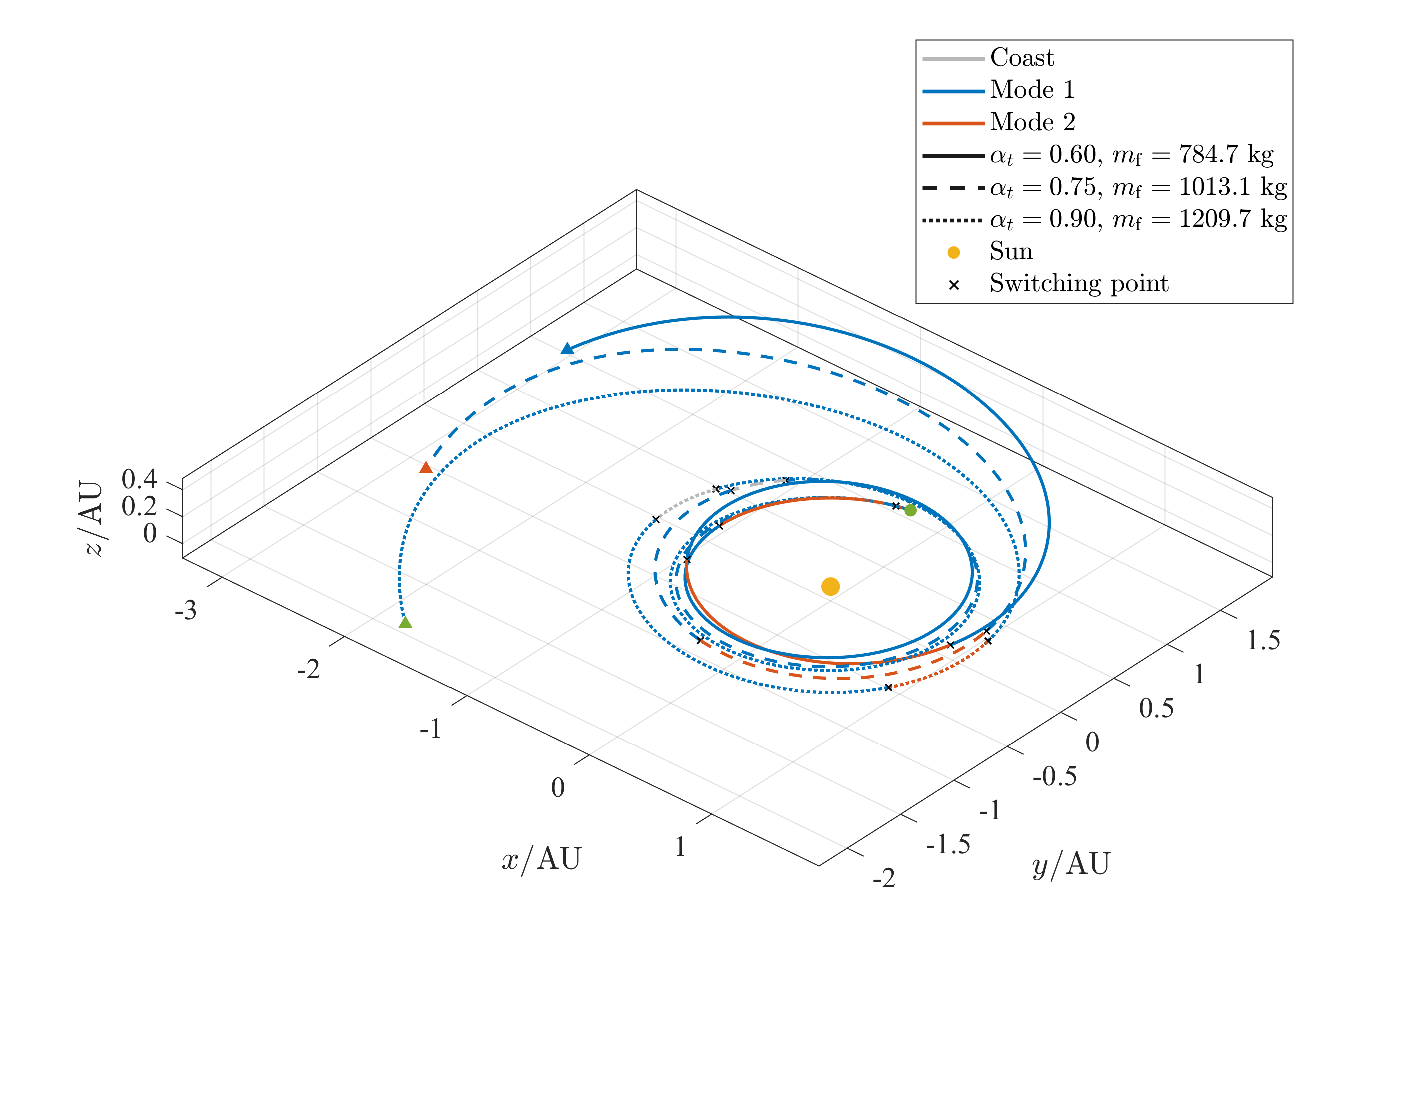
\includegraphics[width=0.98\columnwidth]{pdf_figures/fig3_1_trajectory_3d.pdf}
\caption{Dual-mode coasting transfer trajectories under different $\alpha_t$.}
\label{fig:trajectory-3d}
\end{figure}
The corresponding planar projections in the heliocentric $x$-$y$ plane are shown in Fig.~\ref{fig:trajectory-xy-cases}, which makes the local high-thrust arcs and switching points easier to identify for each transfer-time parameter.

\begin{figure*}[!t]
\centering
\begin{minipage}{0.48\textwidth}
\centering
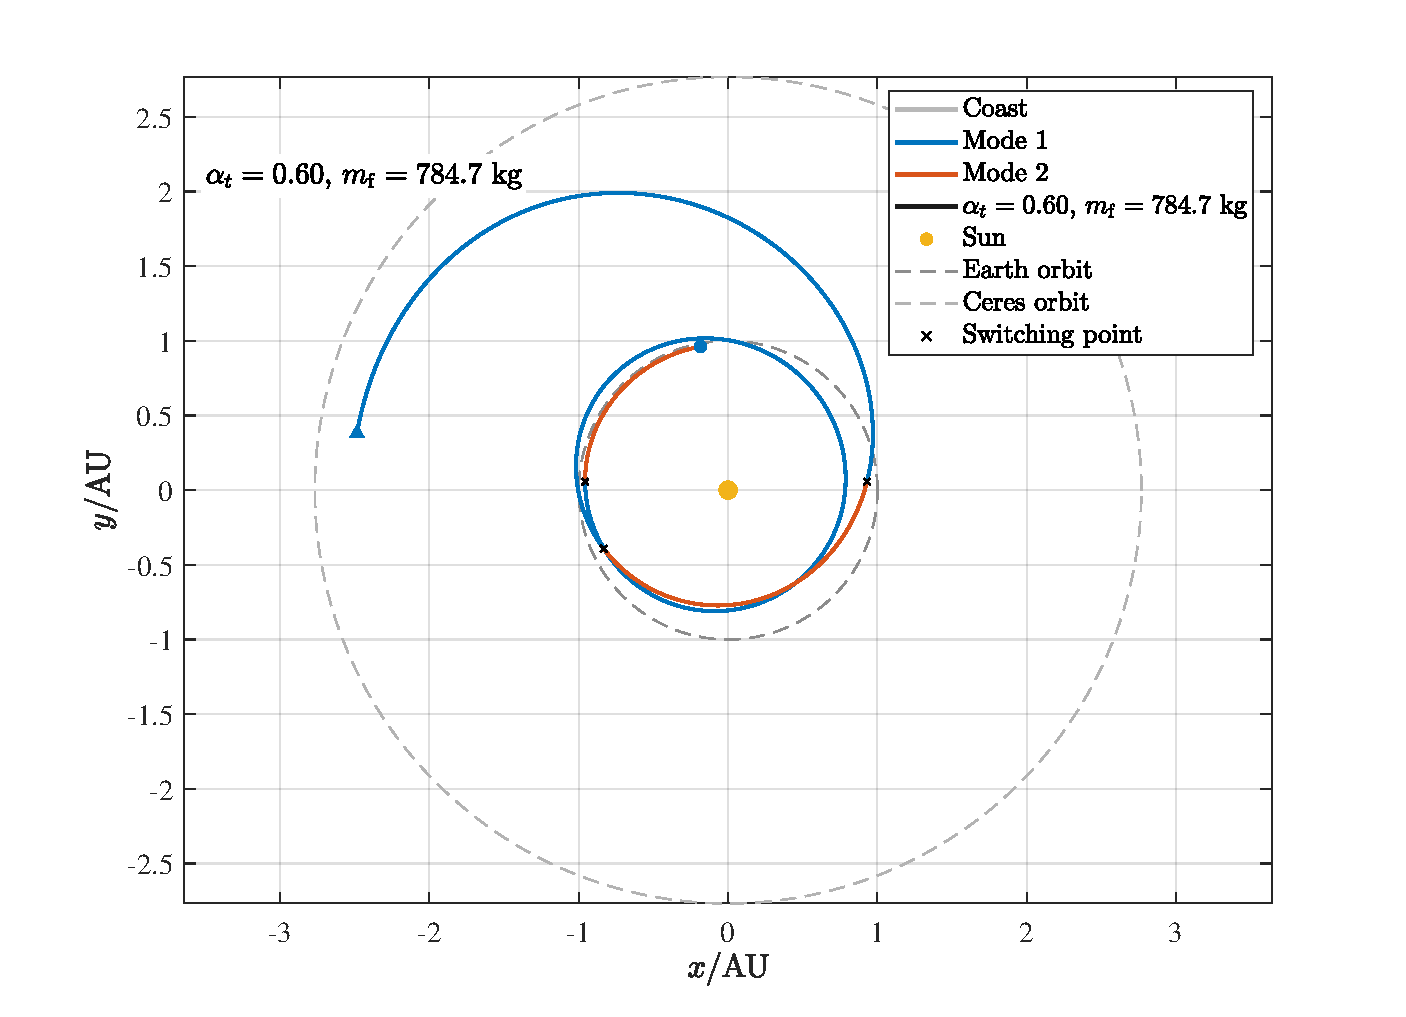
\includegraphics[width=\linewidth]{pdf_figures/fig_02b_trajectory_xy_aa_0p60_mf_0784p651.pdf}\\[-1mm]
\footnotesize (a) $\alpha_t=0.60$.
\end{minipage}\hfill
\begin{minipage}{0.48\textwidth}
\centering
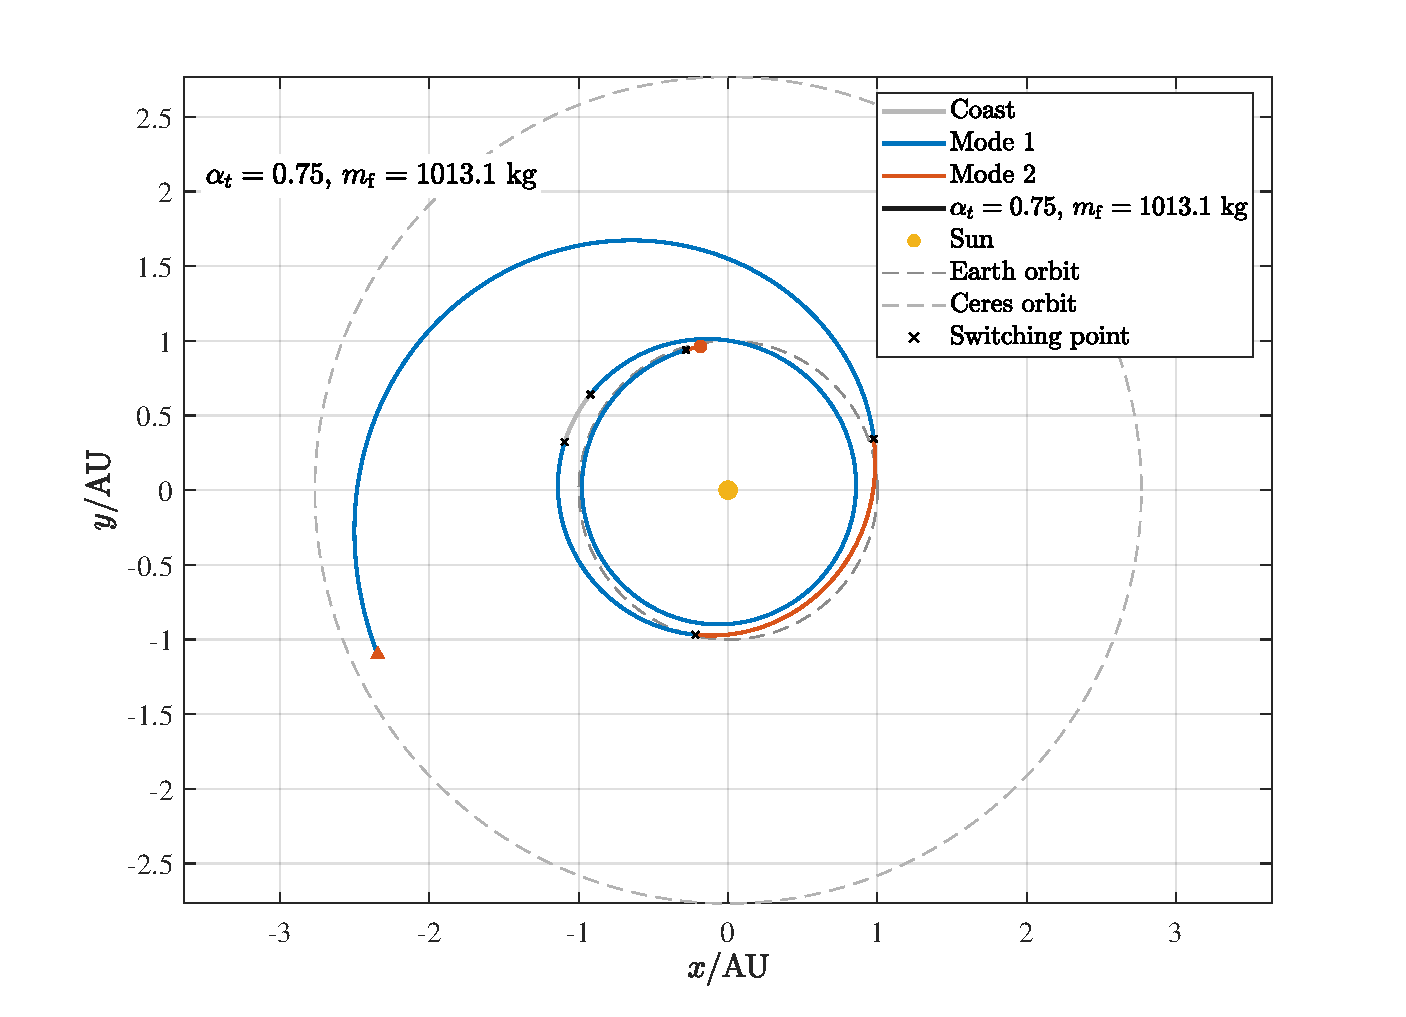
\includegraphics[width=\linewidth]{pdf_figures/fig_02b_trajectory_xy_aa_0p75_mf_1013p061.pdf}\\[-1mm]
\footnotesize (b) $\alpha_t=0.75$.
\end{minipage}
\vspace{1mm}
\begin{minipage}{0.48\textwidth}
\centering
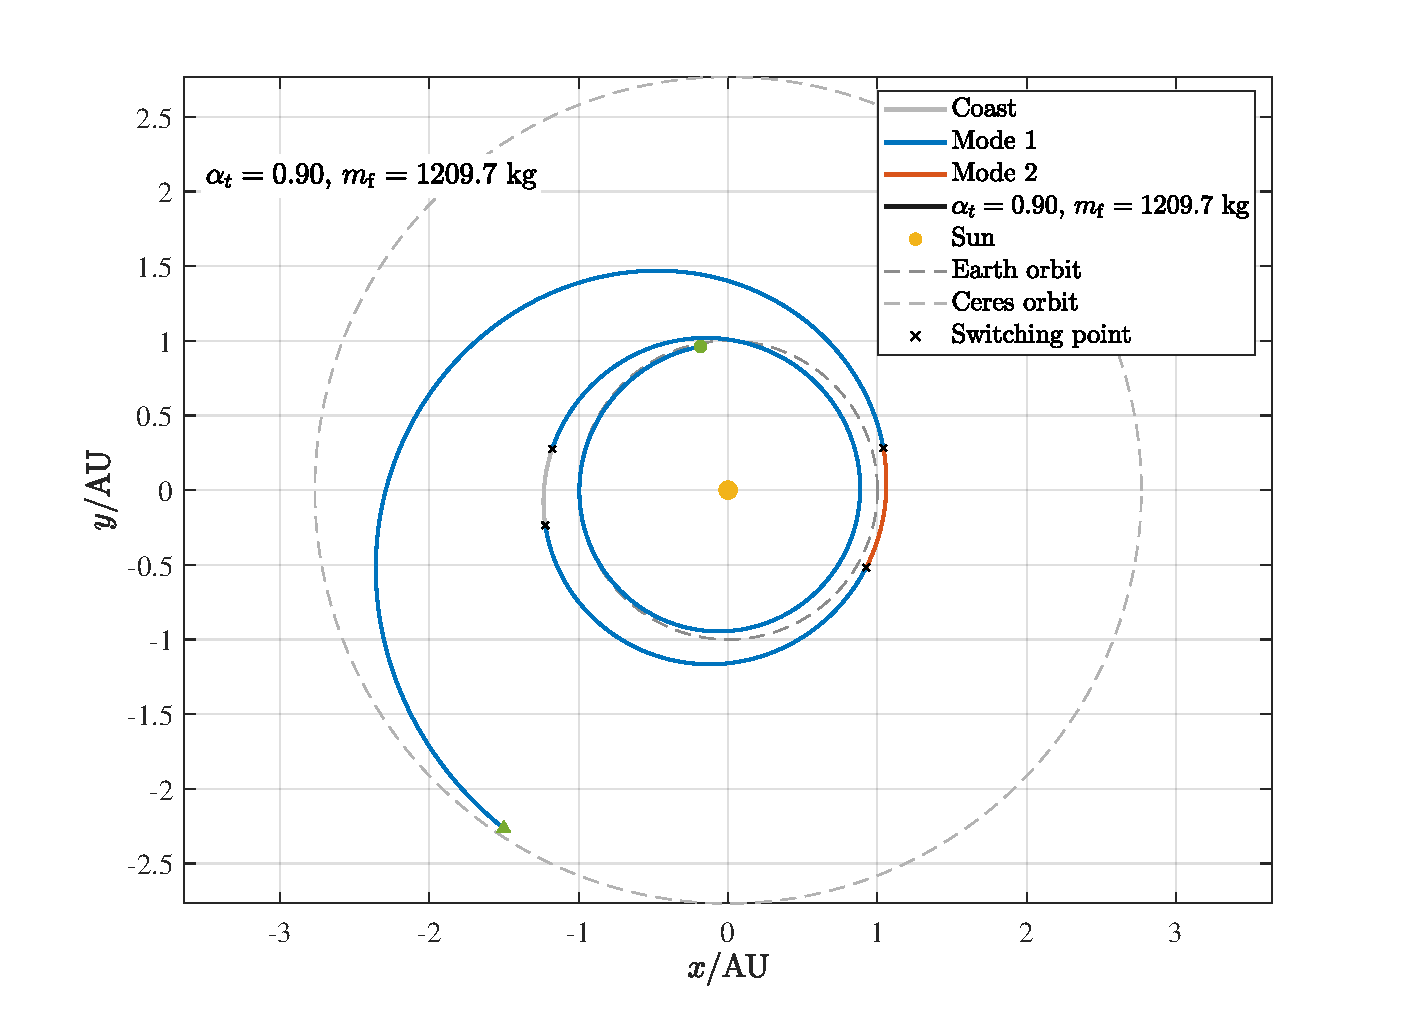
\includegraphics[width=\linewidth]{pdf_figures/fig_02b_trajectory_xy_aa_0p90_mf_1209p719.pdf}\\[-1mm]
\footnotesize (c) $\alpha_t=0.90$.
\end{minipage}
\caption{Heliocentric $x$-$y$ projections of typical dual-mode coasting trajectories under different $\alpha_t$.}
\label{fig:trajectory-xy-cases}
\end{figure*}
All three transfer trajectories show outward expansion from a near-Earth heliocentric orbit to an orbit near Ceres, but the expansion rates are different. For a smaller $\alpha_t$, the orbital-energy increase is more concentrated and the mode-switching points appear earlier in key outward-migration arcs; as $\alpha_t$ increases, the expansion becomes smoother and the low-specific-impulse high-thrust mode is activated only over local short arcs. This indicates that dual-mode optimal control does not distribute thrust between the two modes according to a fixed ratio. Instead, the switching functions determined by the costates call the high-thrust mode only in local intervals where the demands for orbital energy, angular momentum, and plane adjustment are strongest.

\begin{figure}[!hbp]
\centering
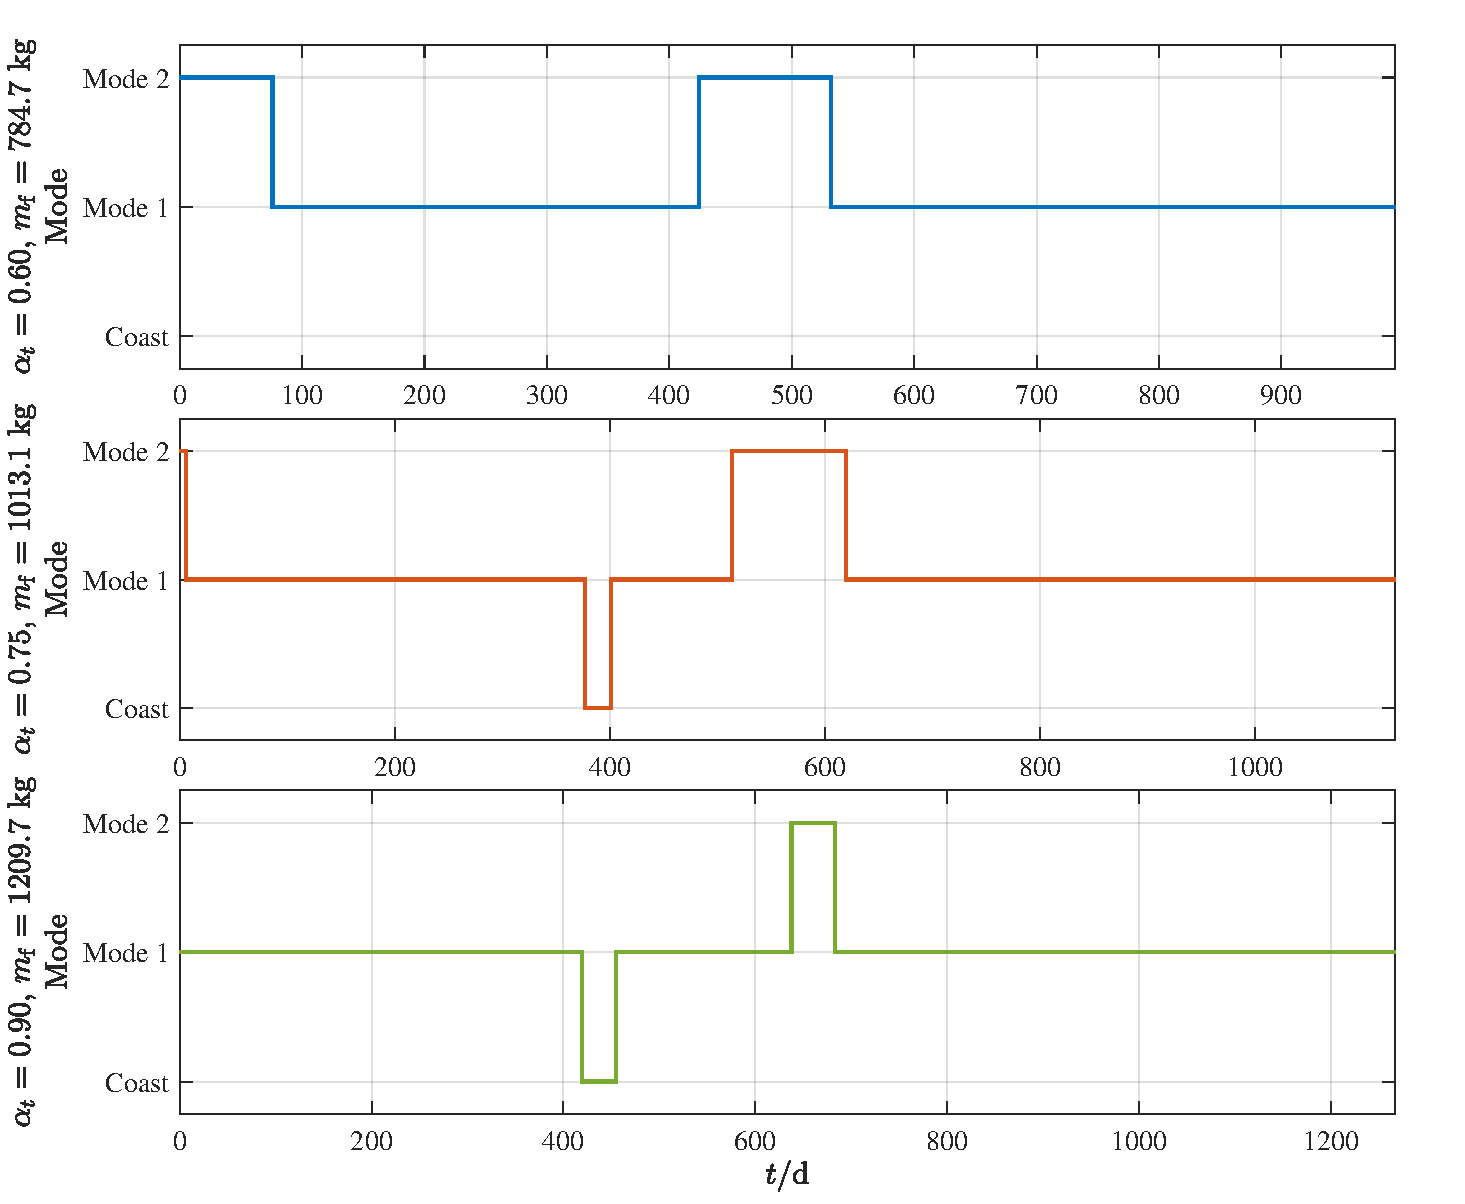
\includegraphics[width=0.98\columnwidth]{pdf_figures/fig3_2_mode_switching.pdf}
\caption{Mode-switching histories of typical cases.}
\label{fig:mode-switching}
\end{figure}

The mode-switching histories further reveal the bang-off-bang structure of the dual-mode coasting solution. The three typical trajectories are all dominated by the high-specific-impulse low-thrust mode, and the high-thrust mode appears only in a few short arcs. For the cases with $\alpha_t=0.75$ and $\alpha_t=0.90$, clear coasting arcs also appear, indicating that continuous thrust over the entire transfer is not necessarily optimal in the fixed-time fuel-optimal problem. When natural drift can complete phase waiting or avoid unnecessary orbital-element perturbations, coasting is directly converted into propellant savings, as shown in more detail in the next subsection.

\begin{figure}[!hbp]
\centering
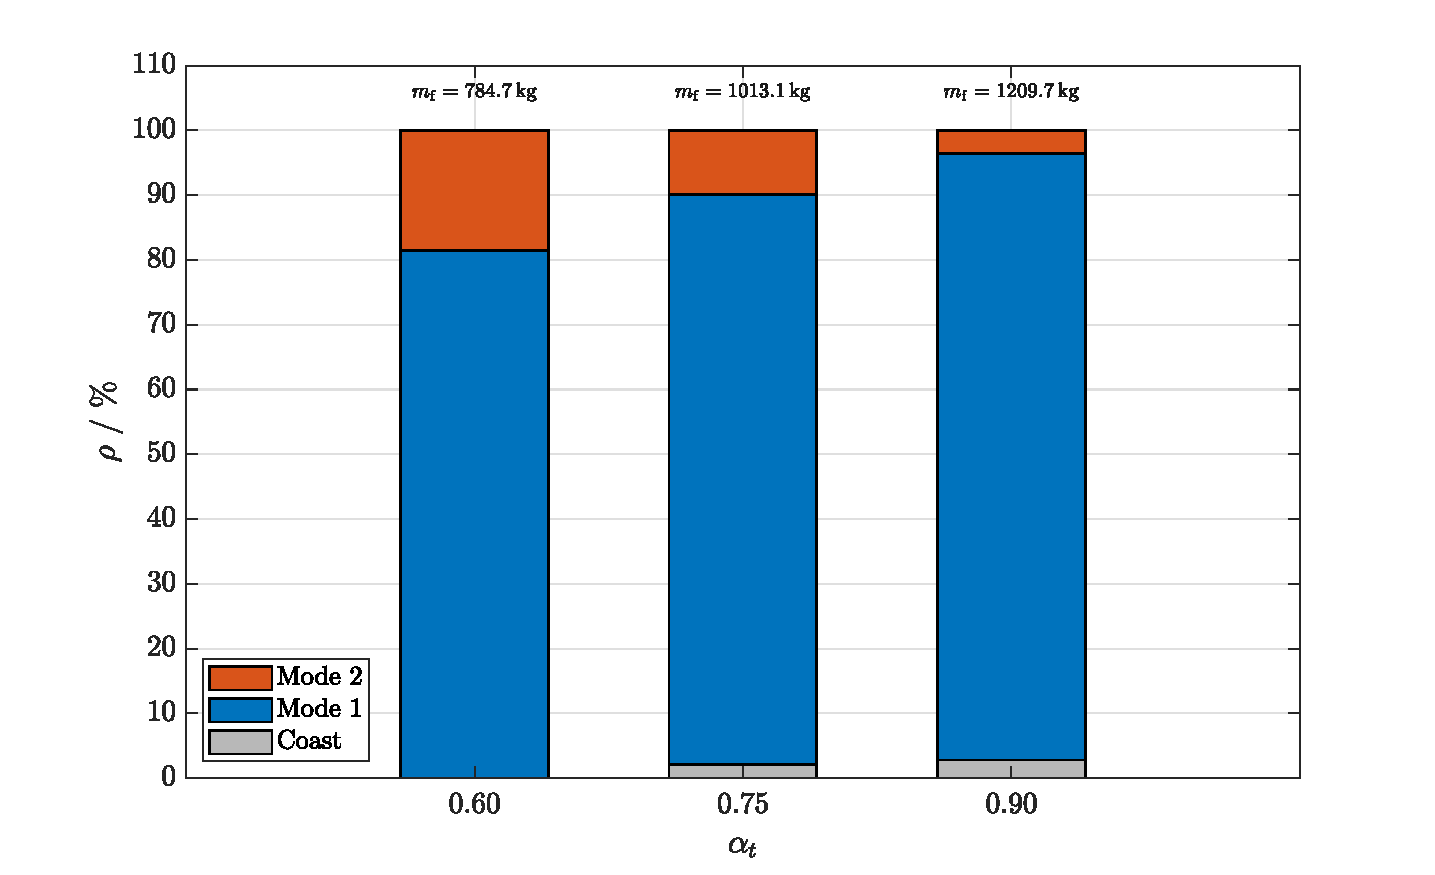
\includegraphics[width=0.98\columnwidth]{pdf_figures/fig3_3_mode_time_mass.pdf}
\caption{Mode-time fractions and terminal mass of typical cases.}
\label{fig:mode-time-mass}
\end{figure}

The mode-time fractions provide a more direct fuel-mechanism interpretation. At $\alpha_t=0.60$, the high-thrust-mode fraction is about 18.56\%, indicating that a short transfer requires stronger rapid maneuvering capability. When $\alpha_t$ increases to 0.90, the high-thrust-mode fraction decreases to 3.58\%, while the low-thrust-mode fraction increases to 93.61\%. This trend is consistent with the increase in terminal mass, showing that the value of the high-thrust mode is mainly to relax time constraints and support local orbital reconstruction, rather than to replace the high-specific-impulse mode in long-duration propulsion.

\begin{figure*}[!t]
\centering
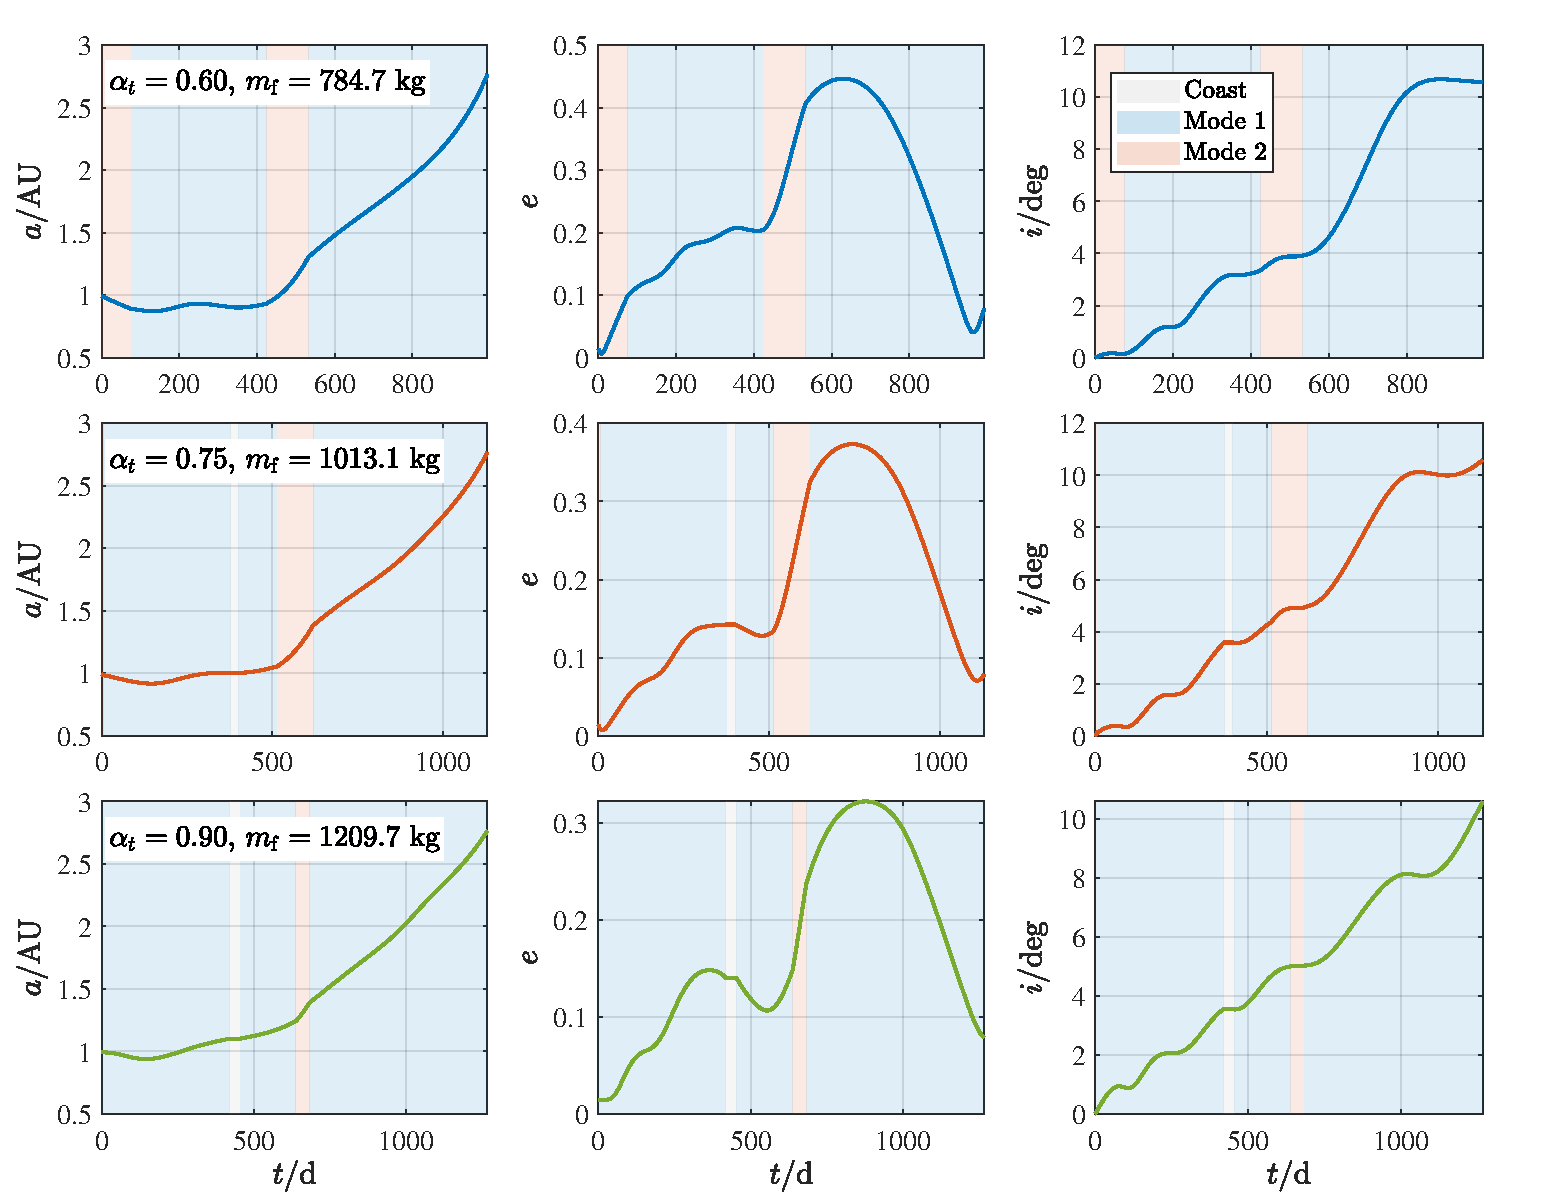
\includegraphics[width=0.88\textwidth]{pdf_figures/fig3_4a_elements_aei.pdf}
\renewcommand{\thefigure}{5a}
\renewcommand{\theHfigure}{5a}
\caption{Variations of semimajor axis, eccentricity, and inclination with mode-activity shading.}
\label{fig:elements-aei}
\end{figure*}

\begin{figure*}[!t]
\centering
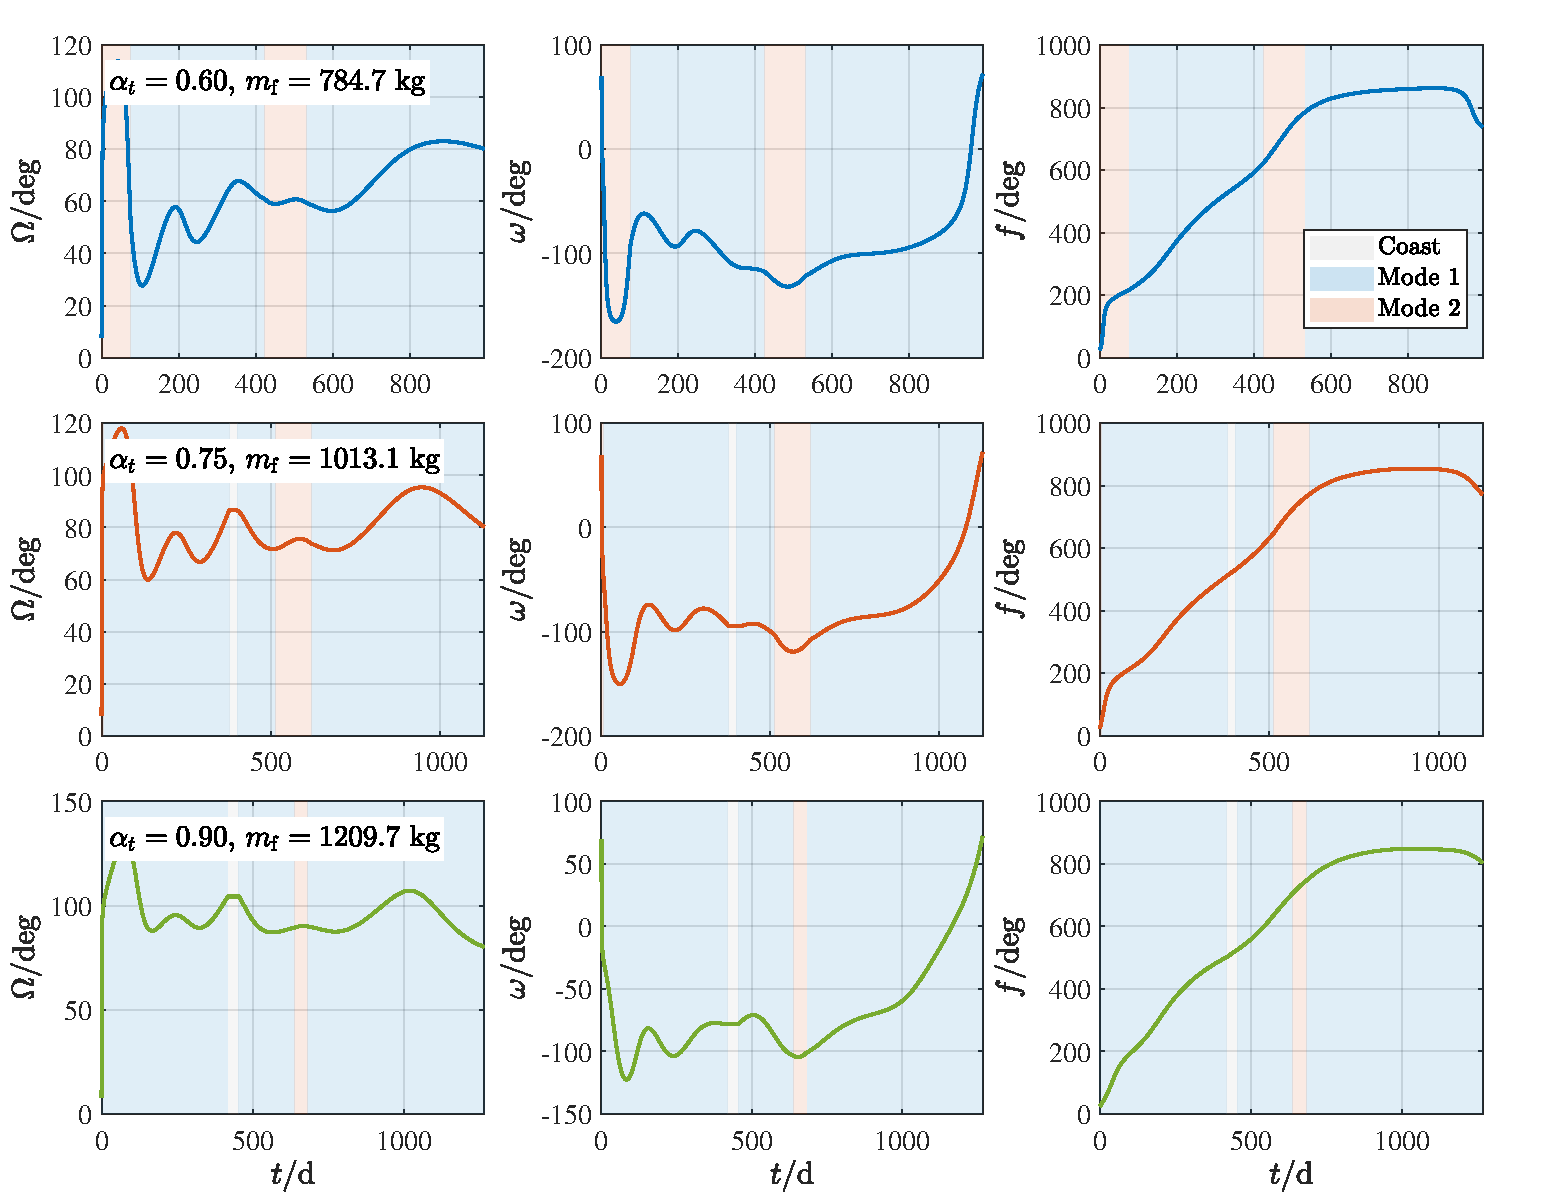
\includegraphics[width=0.88\textwidth]{pdf_figures/fig3_4b_elements_angles.pdf}
\renewcommand{\thefigure}{5b}
\renewcommand{\theHfigure}{5b}
\caption{Variations of RAAN, argument of periapsis, and true anomaly with mode-activity shading.}
\label{fig:elements-angles}
\end{figure*}
\setcounter{figure}{5}
\renewcommand{\thefigure}{\arabic{figure}}
\renewcommand{\theHfigure}{\arabic{figure}}

The orbital-element histories clarify the dynamical causes of mode switching. In Figs.~\ref{fig:elements-aei} and \ref{fig:elements-angles}, the light-blue shading denotes intervals in which mode 1, the low-thrust high-specific-impulse mode, is active; the light-orange shading denotes intervals in which mode 2, the high-thrust low-specific-impulse mode, is active; and unshaded narrow bands denote coasting arcs. The high-thrust shaded intervals usually correspond to rapid semimajor-axis growth or eccentricity adjustment, whereas the coasting arcs mostly appear when the orbital elements vary slowly or when phase matching is required. The gradual inclination variation indicates that the trajectory requires energy increase together with continuous plane correction. The high-thrust mode can accelerate local element variations, but because of its low-specific-impulse penalty, the optimal solution does not use it for long durations. The low-thrust high-specific-impulse mode therefore undertakes most of the energy accumulation and plane-adjustment task.

\subsection{Fuel-Performance Comparison of the Four Propulsion Schemes}
The comparison of the four schemes separates the effects of propulsion operating point and control freedom on fuel performance, rather than serving only as a terminal-mass comparison. The low-thrust-only and high-thrust-only schemes provide performance boundaries for single operating points, whereas the dual-mode coasting and dual-mode noncoasting schemes further examine the effects of mutually exclusive mode selection and coasting freedom. The terminal mass as $\alpha_t$ varies is shown in Fig.~\ref{fig:remaining-mass}, and representative data are listed in Table~\ref{tab:four-schemes}. Fig.~\ref{fig:remaining-mass} shows that the high-thrust-only curve remains at the lowest level, the dual-mode coasting curve is close to or slightly higher than the low-thrust-only curve in the medium-to-long time region, and the dual-mode noncoasting curve drops sharply when $\alpha_t>1$. Although the high-thrust-only scheme has stronger acceleration capability, its low specific impulse makes its overall fuel performance much worse than schemes dominated by the low-thrust high-specific-impulse mode. Its terminal mass remains low, indicating that high thrust without sufficient specific impulse is difficult to translate into fuel advantage in long-duration deep-space transfers. The low-thrust-only scheme can obtain a high terminal mass when enough time is available, and in the interval $\alpha_t=1.00$--1.20 it nearly overlaps the dual-mode coasting scheme. This means that within this time range, the high-specific-impulse low-thrust mode can already complete the main transfer task independently, although its feasibility and rapid maneuvering capability remain limited under tighter time constraints.

\begin{table*}[!t]
\caption{Representative terminal masses of the four schemes (optimal revolution number in parentheses)}
\label{tab:four-schemes}
\centering
\footnotesize
\begin{tabular}{ccccc}
\toprule
$\alpha_t$ & Low-thrust only/kg & High-thrust only/kg & Dual-mode with coasting/kg & Dual-mode without coasting/kg \\
\midrule
0.60 & -- & 550.4(1) & 1098.3(1) & 1040.4(1) \\
0.75 & -- & 553.7(1) & 1100.5(1) & 1012.6(2) \\
0.90 & -- & 556.1(1) & 1209.7(2) & 1207.9(2) \\
1.00 & 1323.2(2) & 574.2(2) & 1325.0(2) & 1323.2(2) \\
1.10 & 1413.7(2) & 591.9(2) & 1413.7(2) & 919.5(1) \\
1.20 & 1451.6(2) & 591.9(2) & 1451.6(2) & 904.7(1) \\
\bottomrule
\end{tabular}
\end{table*}

\begin{figure}[!hbp]
\centering
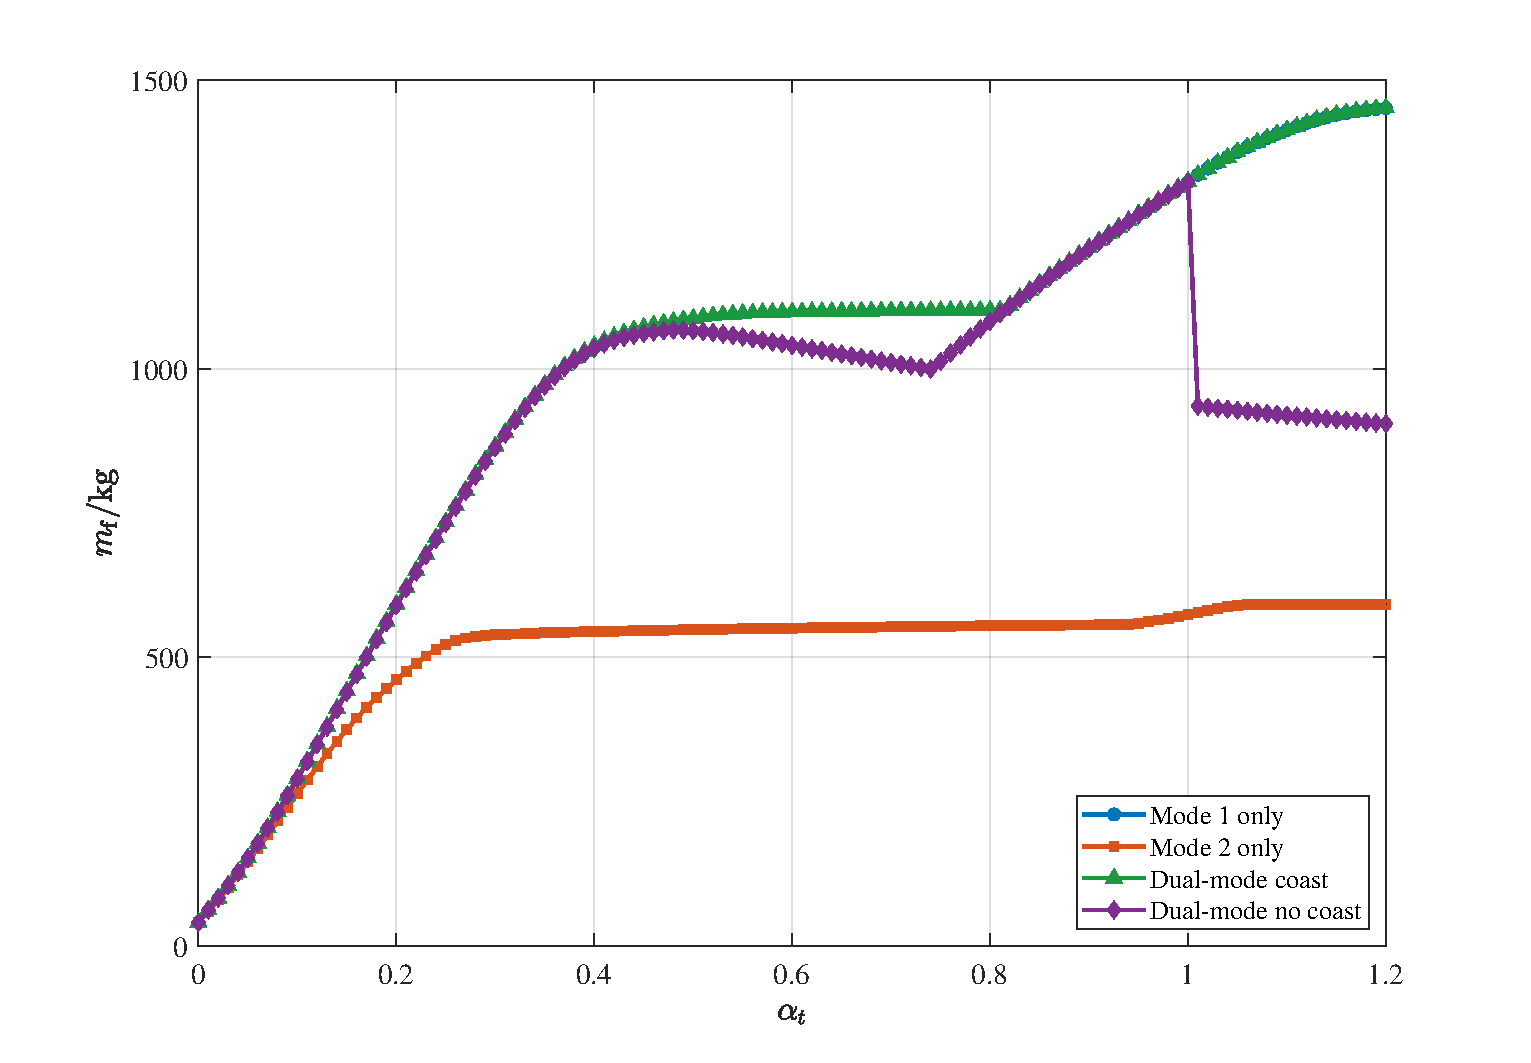
\includegraphics[width=0.98\columnwidth]{pdf_figures/fig3_5_remaining_mass.pdf}
\caption{Terminal mass of the four propulsion schemes as a function of $\alpha_t$.}
\label{fig:remaining-mass}
\end{figure}

\begin{figure}[!hbp]
\centering
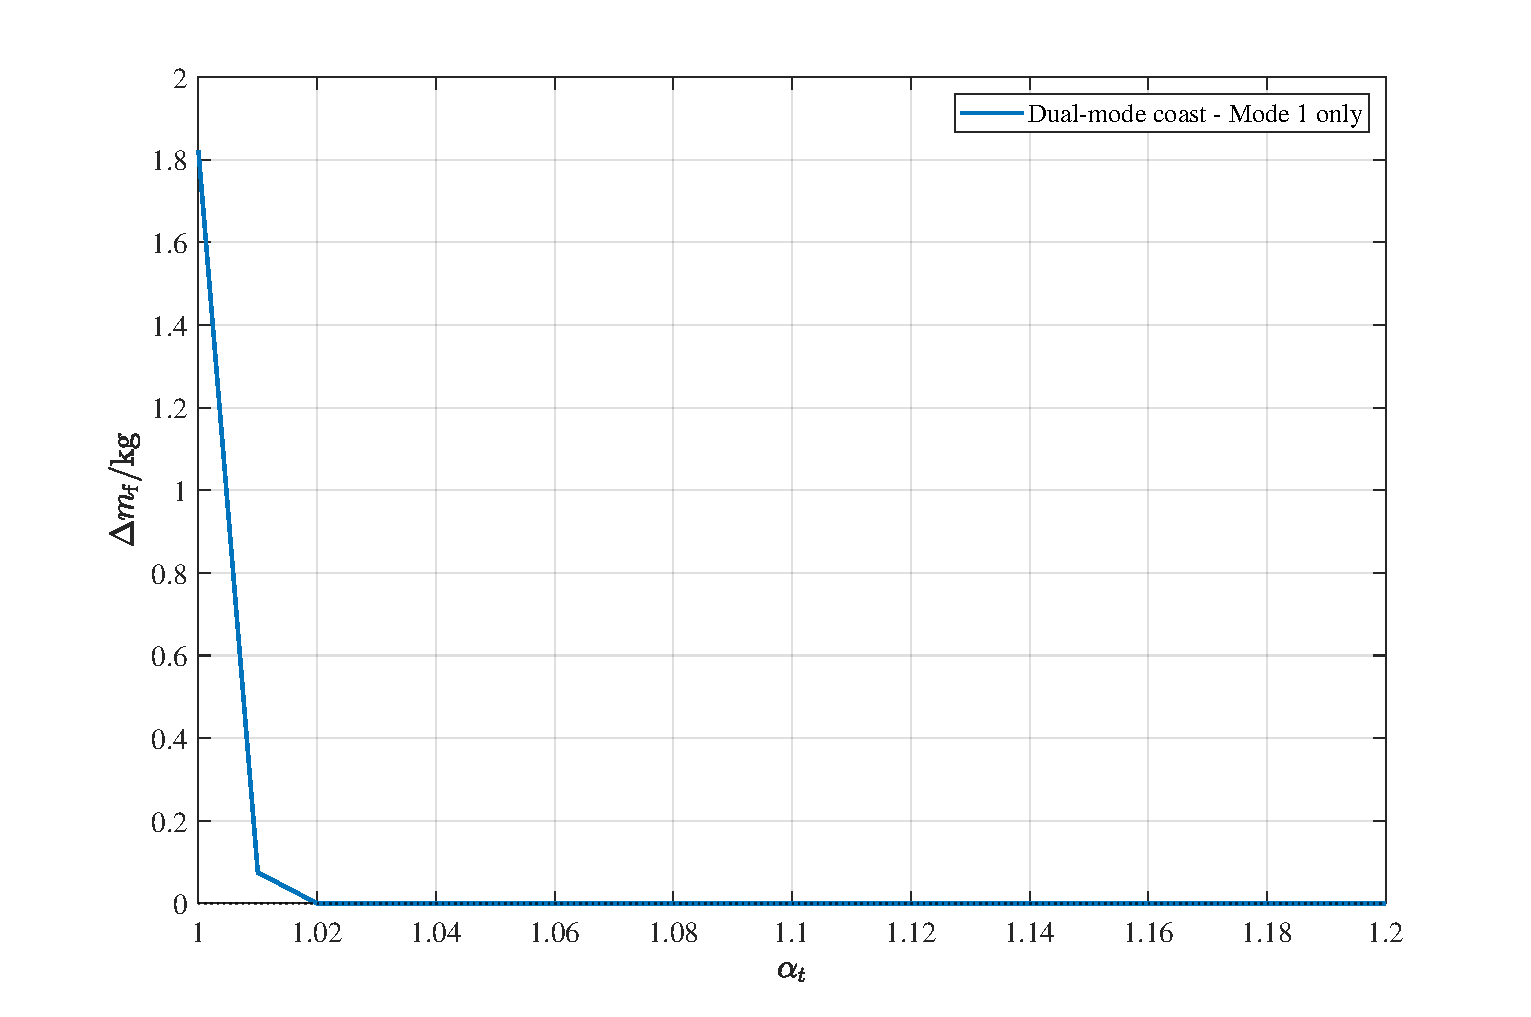
\includegraphics[width=0.98\columnwidth]{pdf_figures/fig3_6_gain_vs_low_thrust.pdf}
\caption{Terminal-mass gain of the dual-mode coasting scheme relative to the low-thrust-only scheme.}
\label{fig:gain-low-thrust}
\end{figure}

\begin{figure}[!hbp]
\centering
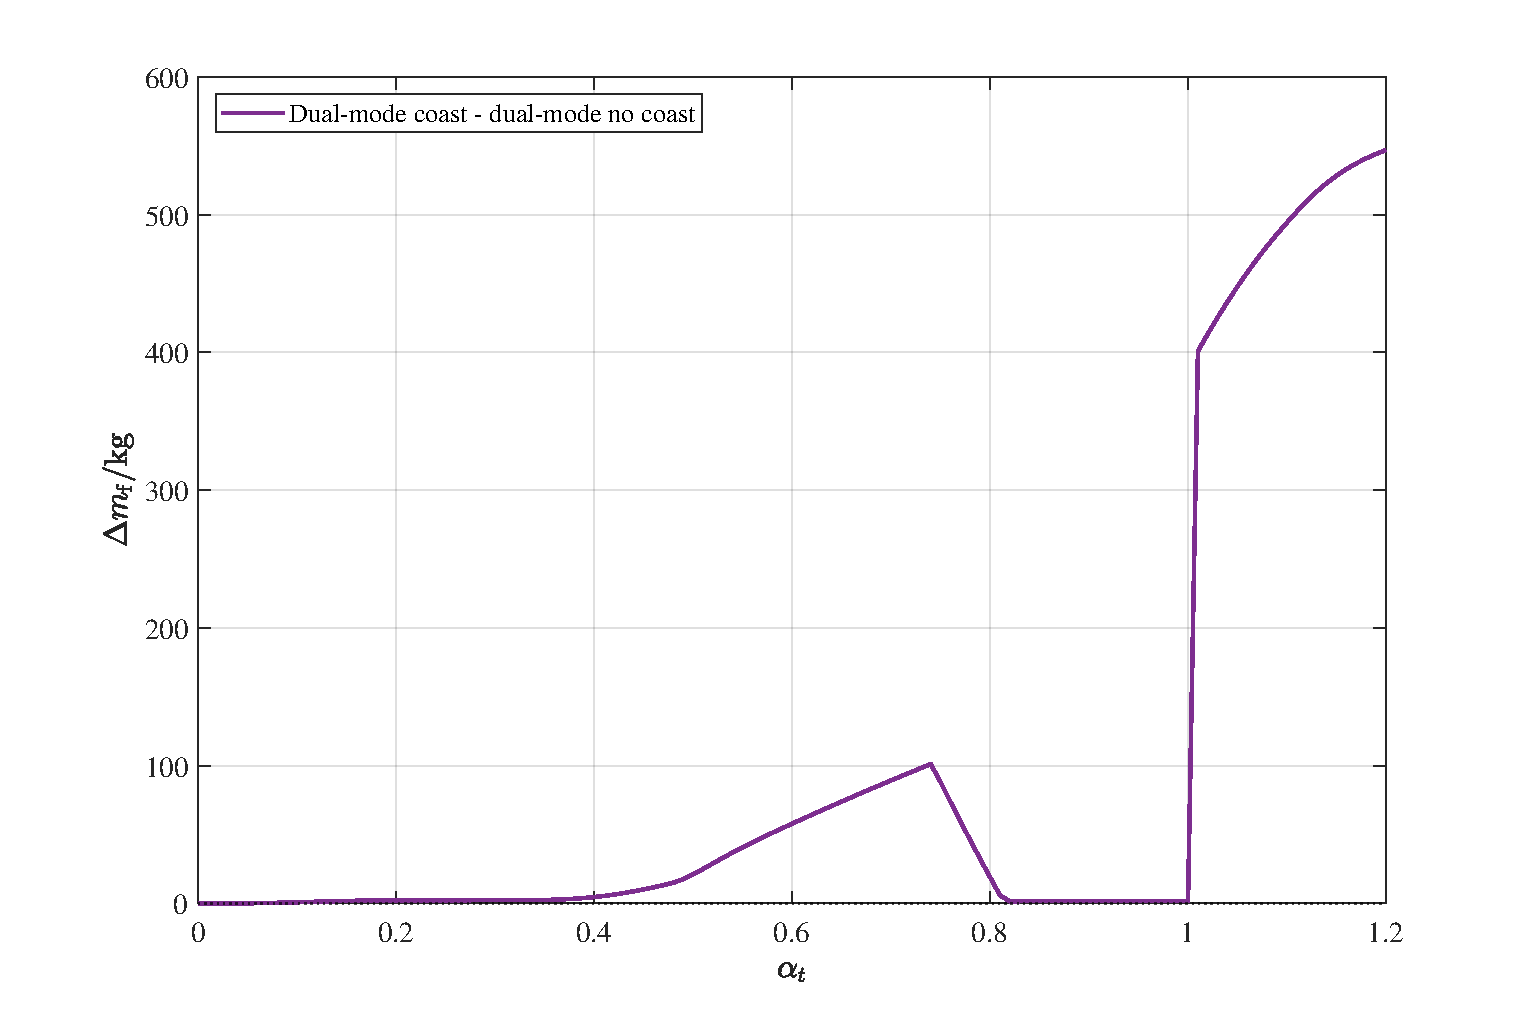
\includegraphics[width=0.98\columnwidth]{pdf_figures/fig3_7_gain_vs_noncoast.pdf}
\caption{Terminal-mass gain of the dual-mode coasting scheme relative to the dual-mode noncoasting scheme.}
\label{fig:gain-noncoast}
\end{figure}

The dual-mode coasting scheme nearly overlaps the low-thrust-only scheme in the interval $\alpha_t=1.00$--1.20. At $\alpha_t=1.00$, its terminal-mass gain relative to the low-thrust-only scheme is about 1.822 kg, whereas at $\alpha_t=1.10$ and $\alpha_t=1.20$ the terminal masses of the two schemes listed in Table~\ref{tab:four-schemes} are identical. This overlap indicates that when the transfer time approaches or exceeds the all-low-thrust time-optimal baseline, mode 1 can independently complete the main energy accumulation and phase adjustment. The high-thrust low-specific-impulse mode no longer provides a clear net benefit, and the dual-mode coasting optimum automatically degenerates into a solution dominated by the low-thrust mode. In contrast, the dual-mode noncoasting curve exhibits a distinct jump after $\alpha_t>1$ because this scheme enforces thrust over the entire transfer and cannot use the extra time for natural drift and phase waiting. Table~\ref{tab:four-schemes} also shows that its optimal revolution number switches from two revolutions to one revolution, changing the control structure and orbital winding pattern. The discontinuous terminal-mass decrease indicates that coasting freedom is decisive for the fuel-optimal solution in long time windows.

Coasting freedom has a pronounced influence on the fixed-time fuel-optimal problem. At $\alpha_t=1.20$, the terminal mass of the dual-mode coasting scheme is 1451.641 kg, whereas that of the dual-mode noncoasting scheme is only 904.694 kg. Although the latter also has two thrust modes, it consumes unnecessary propellant in long-duration transfer because thrust must be applied throughout the trajectory. This result indicates that the advantage of dual-mode propulsion is tied to the combined choice among thrusting, coasting, and operating mode, rather than merely to the presence of an additional mode.

\begin{figure}[!hbp]
\centering
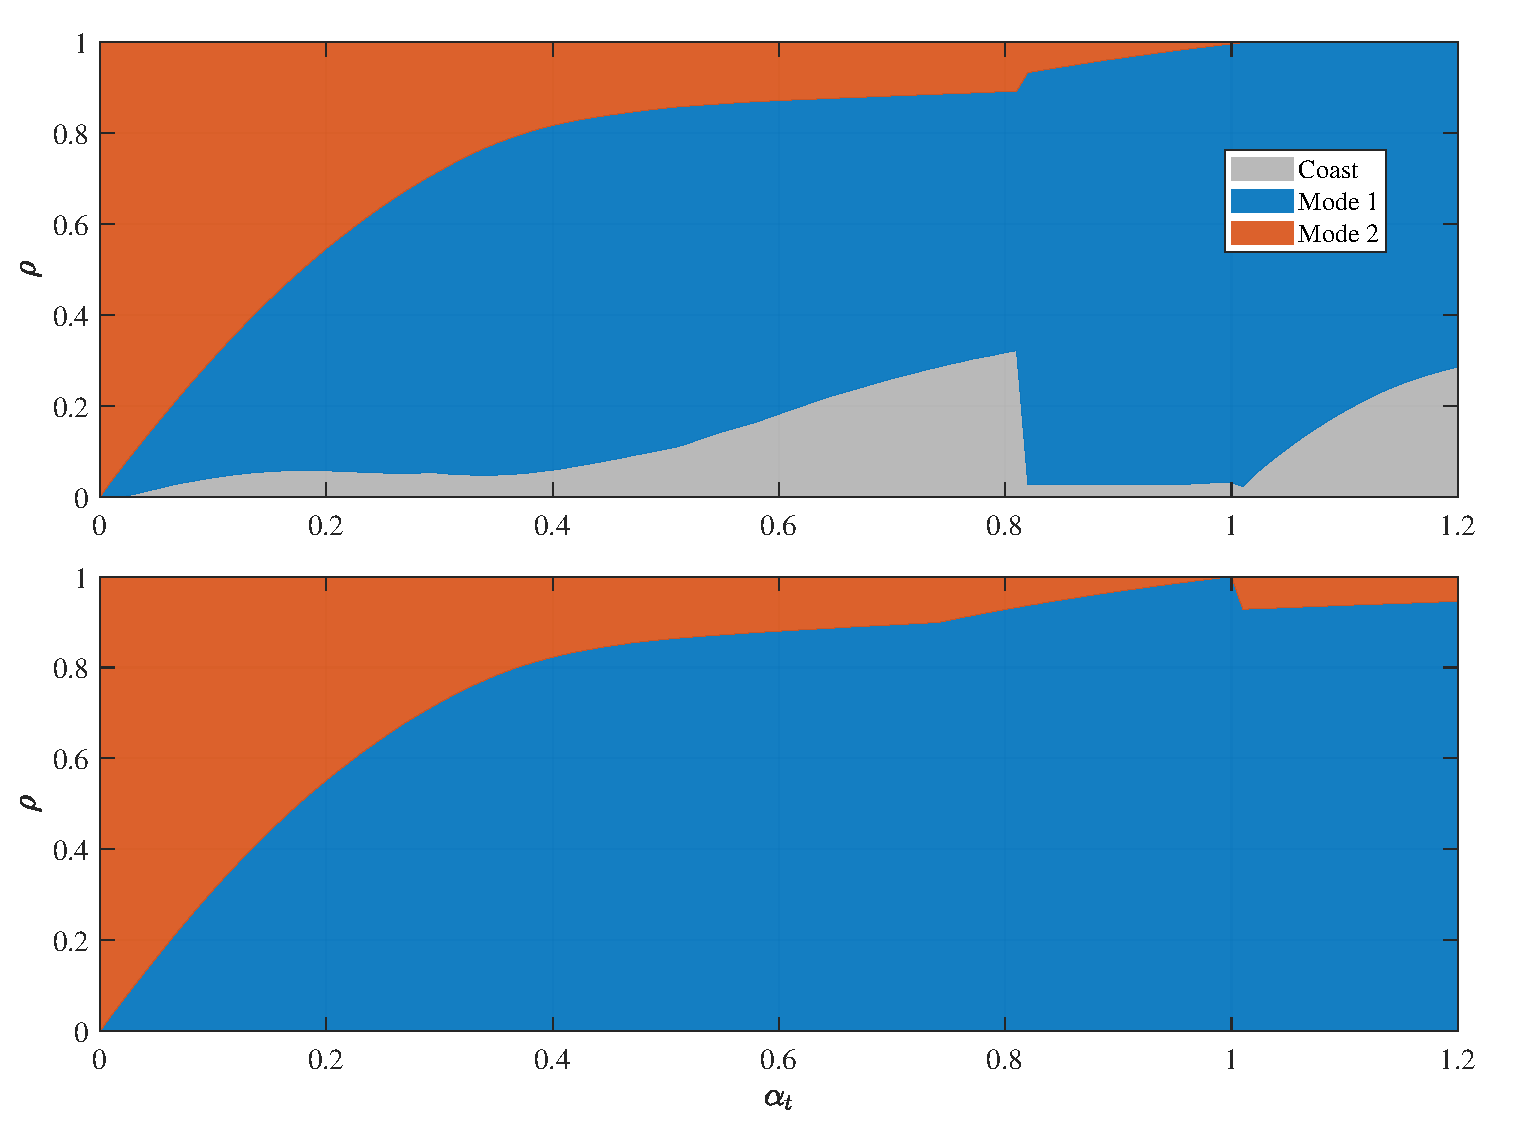
\includegraphics[width=0.98\columnwidth]{pdf_figures/fig3_8_mode_fractions.pdf}
\caption{Mode-time fractions of the dual-mode schemes as $\alpha_t$ varies.}
\label{fig:mode-fractions}
\end{figure}

The mode fractions provide a direct explanation for these performance differences. The dual-mode coasting scheme exhibits clear coasting arcs under medium and larger $\alpha_t$, whereas the dual-mode noncoasting scheme can only switch between the two propulsion modes and cannot use natural drift to save propellant. When a longer transfer time is allowed, forced continuous thrust destroys the fuel advantage of phase-waiting intervals. When the mission time is tight, the high-thrust mode provides the necessary rapid maneuvering capability. The thrust/coast sequence in dual-mode trajectory design should therefore not be prescribed in advance. It is determined by the switching functions and mode Hamiltonians, and dual-mode propulsion should not be interpreted simply as continuous alternation between two modes.

\subsection{Two-Dimensional Critical Boundary Analysis}
Under the baseline dual-mode parameters, the fuel advantage of the dual-mode coasting scheme over the low-thrust-only scheme is small, making propulsion-parameter matching critical. The low-thrust-only result with $\alpha_t=1.00$ and two revolutions is used as the baseline, with a terminal mass of 1323.215004 kg. With the low-thrust-mode parameters fixed, the two-dimensional parameters $(r_{\mathrm{T}},r_{\mathrm{I}})$ are varied, and the terminal-mass gain of the dual-mode coasting scheme is computed in the two-dimensional plane formed by the thrust ratio and the specific-impulse ratio. This representation avoids compressing the four propulsion parameters into a single composite index and is more suitable for observing the coupled relation between thrust enhancement and specific-impulse loss.

\begin{figure}[!t]
\centering
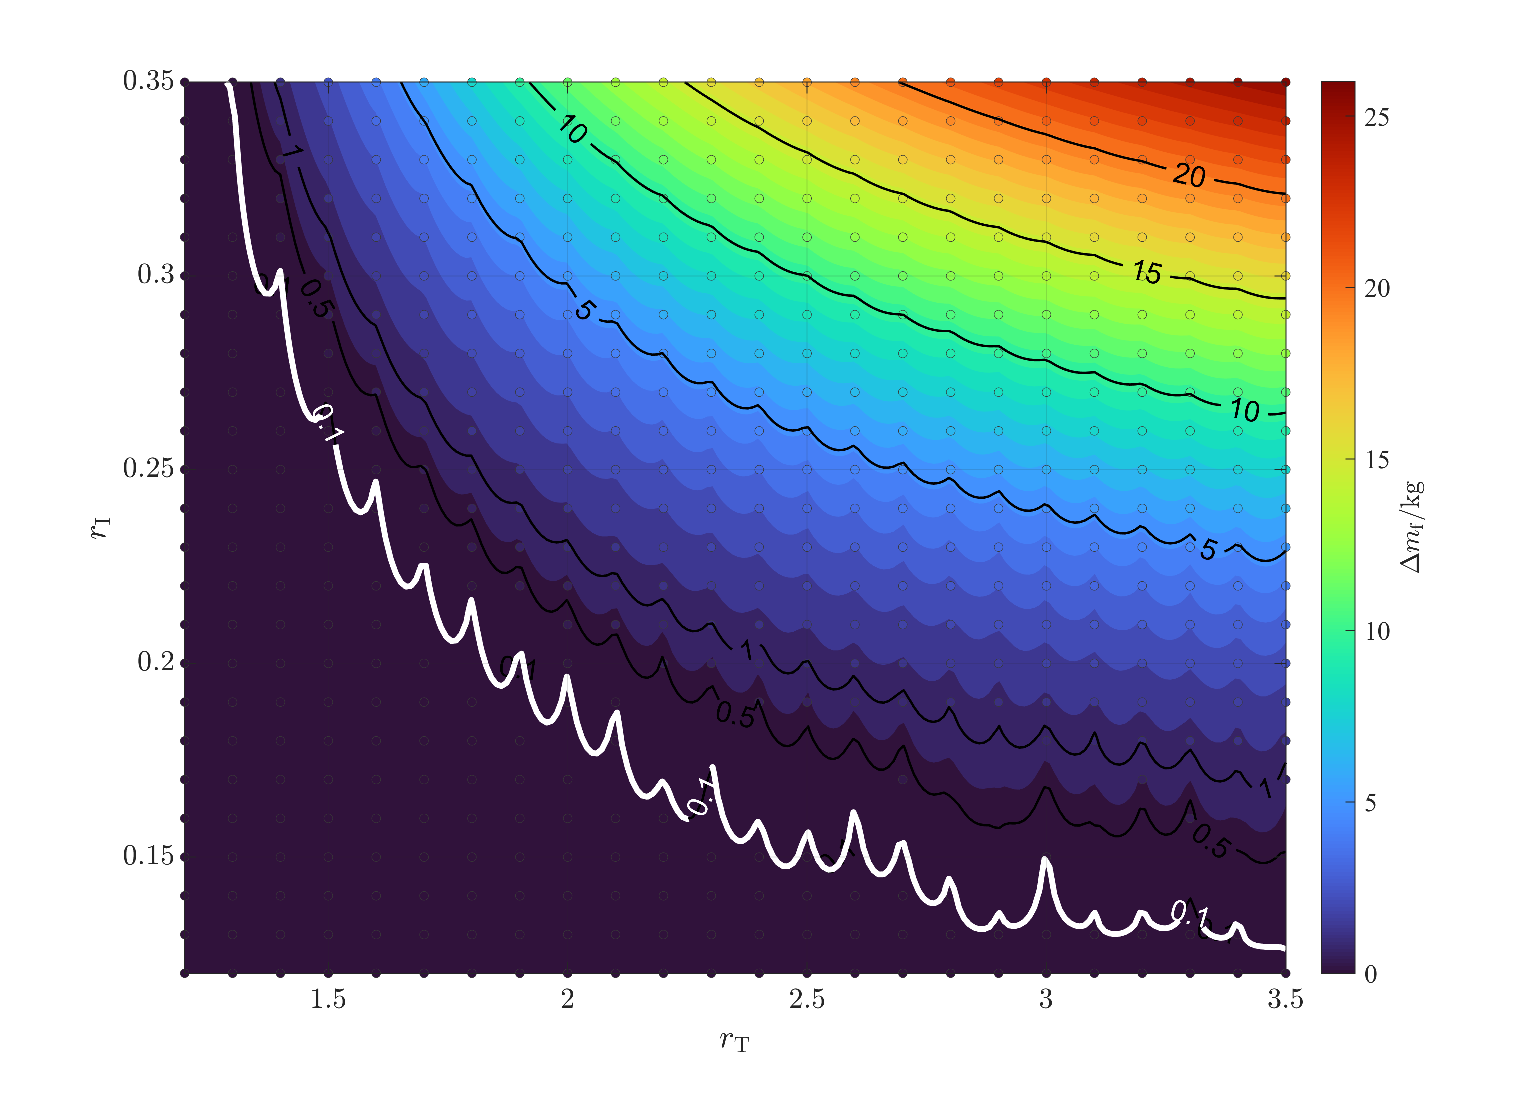
\includegraphics[width=0.98\columnwidth]{pdf_figures/fig3_9_mass_gain_boundary.pdf}
\caption{Dual-mode mass gain and critical boundary in the thrust-ratio-specific-impulse-ratio plane.}
\label{fig:mass-gain-boundary}
\end{figure}

The continuously interpolated mass-gain $\Delta m_{\mathrm{f}}$ distribution shows that the lower-left region has zero mass gain, whereas the upper-right region contains positive gains. The dual-mode advantage boundary is inclined overall from the low-thrust-ratio, high-specific-impulse-ratio region toward the high-thrust-ratio, low-specific-impulse-ratio region. This trend indicates that when the thrust advantage of the high-thrust mode is weak, its specific impulse must remain close to that of the low-thrust mode to offset the propellant penalty. As the thrust ratio increases, the high-thrust mode can complete local orbital reconstruction in a shorter time, and the required specific-impulse ratio is therefore reduced. The maximum mass gain appears near a thrust ratio of 3.50 and a specific-impulse ratio of 0.35, with a gain of about 25.619 kg and a corresponding terminal mass of 1348.834 kg.

\begin{figure}[!t]
\centering
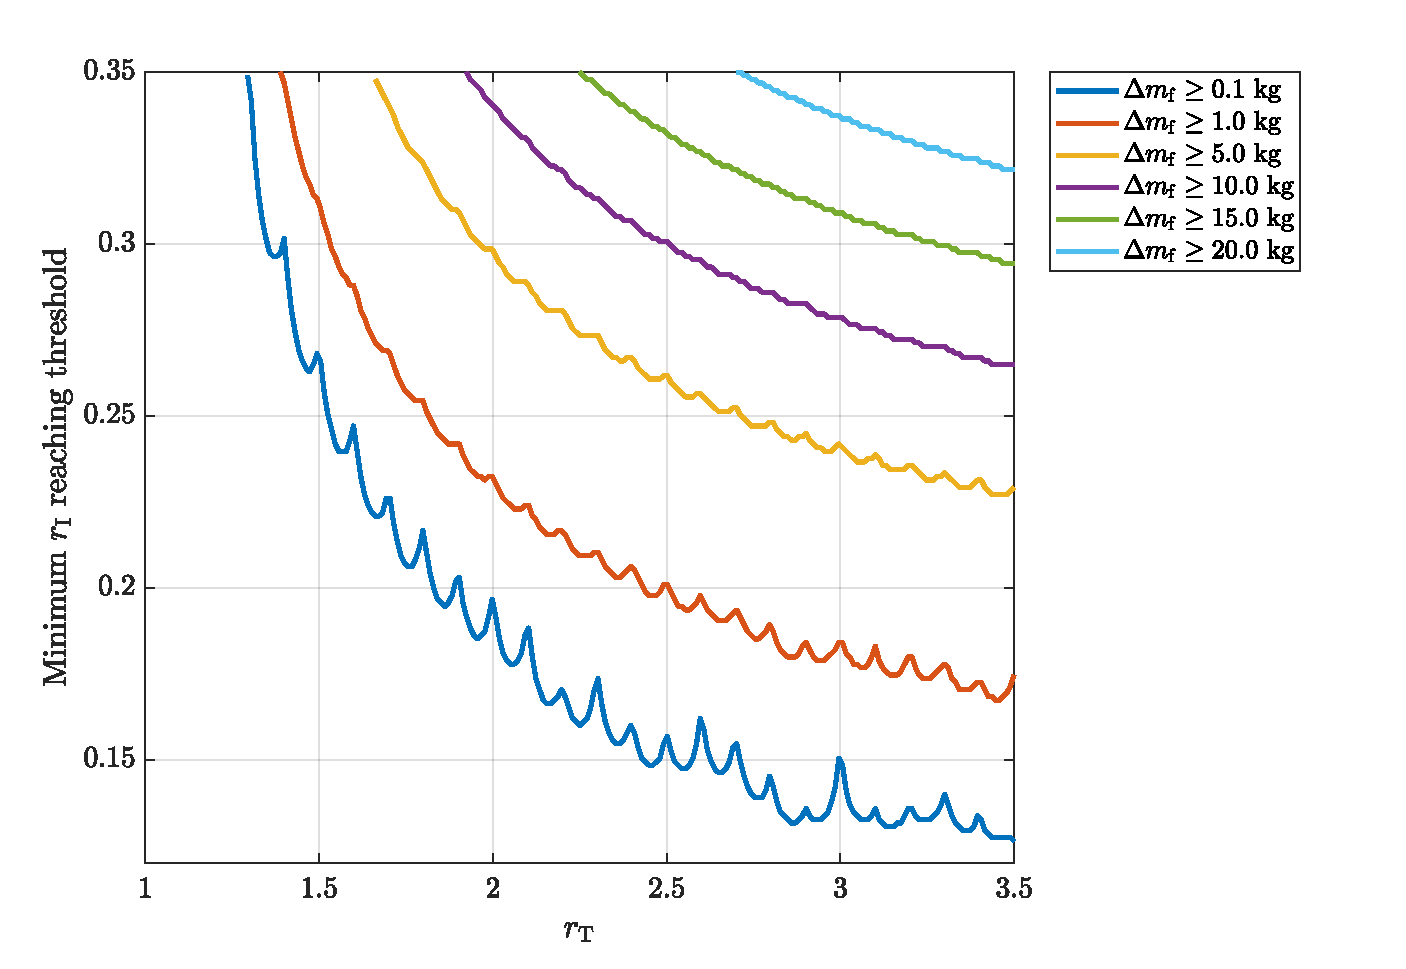
\includegraphics[width=0.98\columnwidth]{pdf_figures/fig3_10_threshold_curves.pdf}
\caption{Minimum specific-impulse-ratio curves corresponding to different mass-gain thresholds.}
\label{fig:threshold-curves}
\end{figure}

The mass-gain-threshold $B_{\varepsilon}$ curves further transform the two-dimensional results into propulsion-parameter selection criteria. For a small gain on the order of 1 kg, increasing the thrust ratio reduces the required specific-impulse ratio. For gains greater than 10 kg, the curves shrink noticeably toward the high-specific-impulse-ratio region, indicating that large benefits require not only high thrust capability but also a sufficiently high specific impulse in the high-thrust mode. The parameter region satisfying a mass gain no smaller than $\Delta m_{\mathrm{f}}=1~\mathrm{kg}$ accounts for about 57.17\%, the region satisfying no smaller than $\Delta m_{\mathrm{f}}=5~\mathrm{kg}$ accounts for about 18.99\%, and the region satisfying no smaller than $\Delta m_{\mathrm{f}}=10~\mathrm{kg}$ accounts for only about 3.68\%. A high-benefit dual-mode scheme therefore requires high thrust together with an acceptable specific-impulse penalty.

\begin{figure}[!t]
\centering
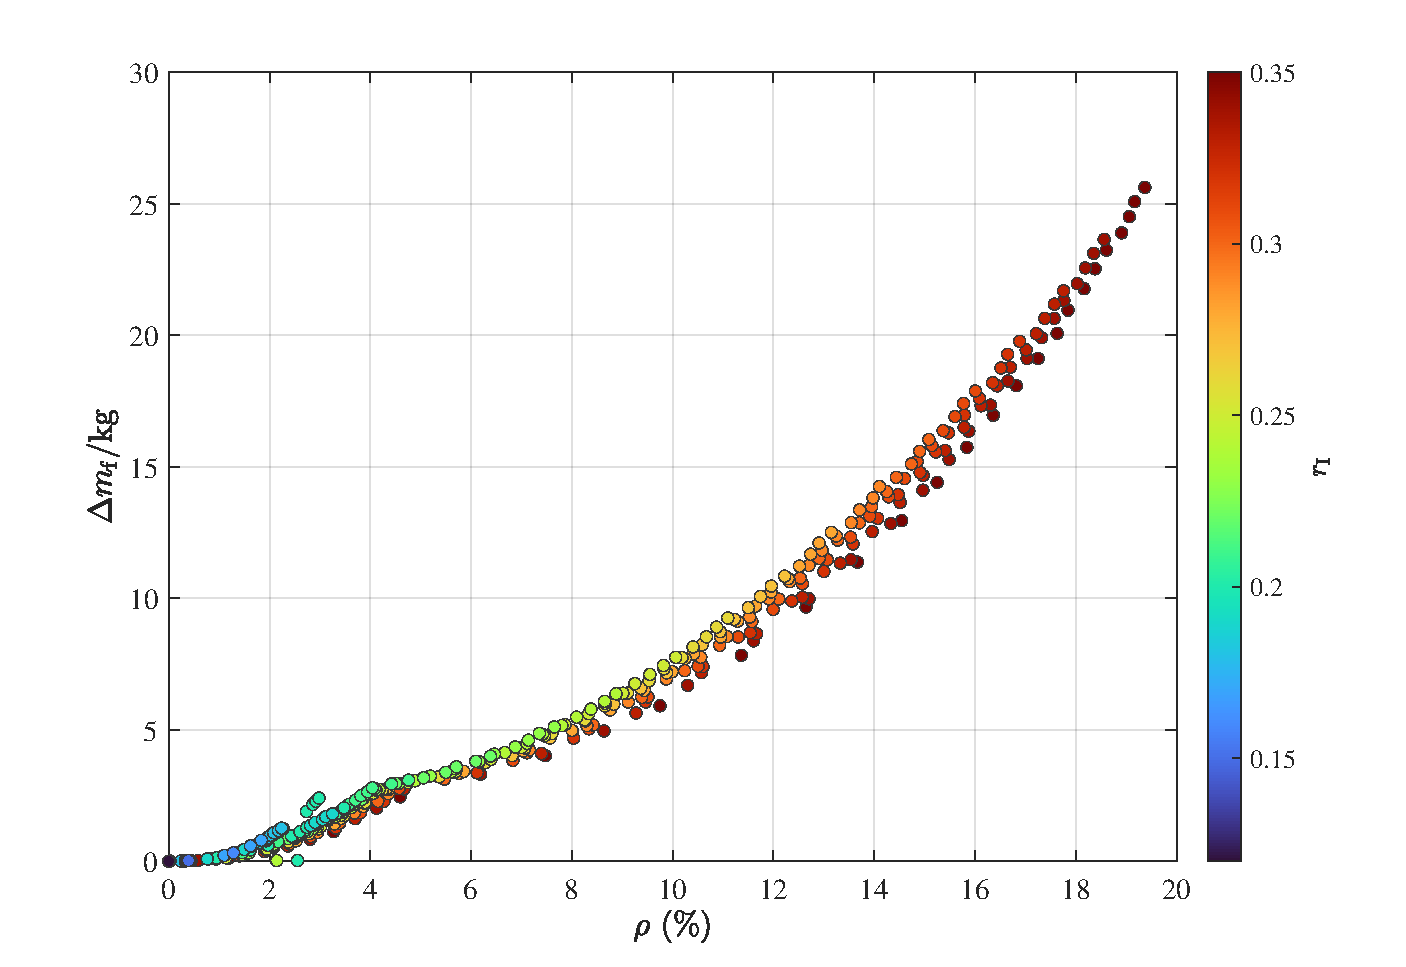
\includegraphics[width=0.98\columnwidth]{pdf_figures/fig3_11_gain_vs_fraction.pdf}
\caption{Relationship between the non-low-thrust mode fraction $\rho$ and mass gain $\Delta m_{\mathrm{f}}$.}
\label{fig:gain-fraction}
\end{figure}

From the perspective of mode usage, the non-low-thrust mode fraction $\rho$ and the mass gain $\Delta m_{\mathrm{f}}$ show a strong correlation, with a correlation coefficient of about 0.969. The correlation coefficient between the high-thrust-mode fraction and the mass gain is about 0.873. This indicates that the mass benefit of dual-mode propulsion does not come from simply extending the high-thrust operation time, but from the combination of short high-thrust maneuvers and necessary coasting. The point with the largest high-thrust-mode fraction is located near a thrust ratio of 2.10 and a specific-impulse ratio of 0.35, where the high-thrust-mode fraction is about 2.12\%. However, this point is not the maximum mass-gain point. Thus, optimal mode selection is governed by the balance between orbital-dynamics benefit and propellant consumption, rather than by a monotonic preference for longer high-thrust operation.

\begin{figure}[!t]
\centering
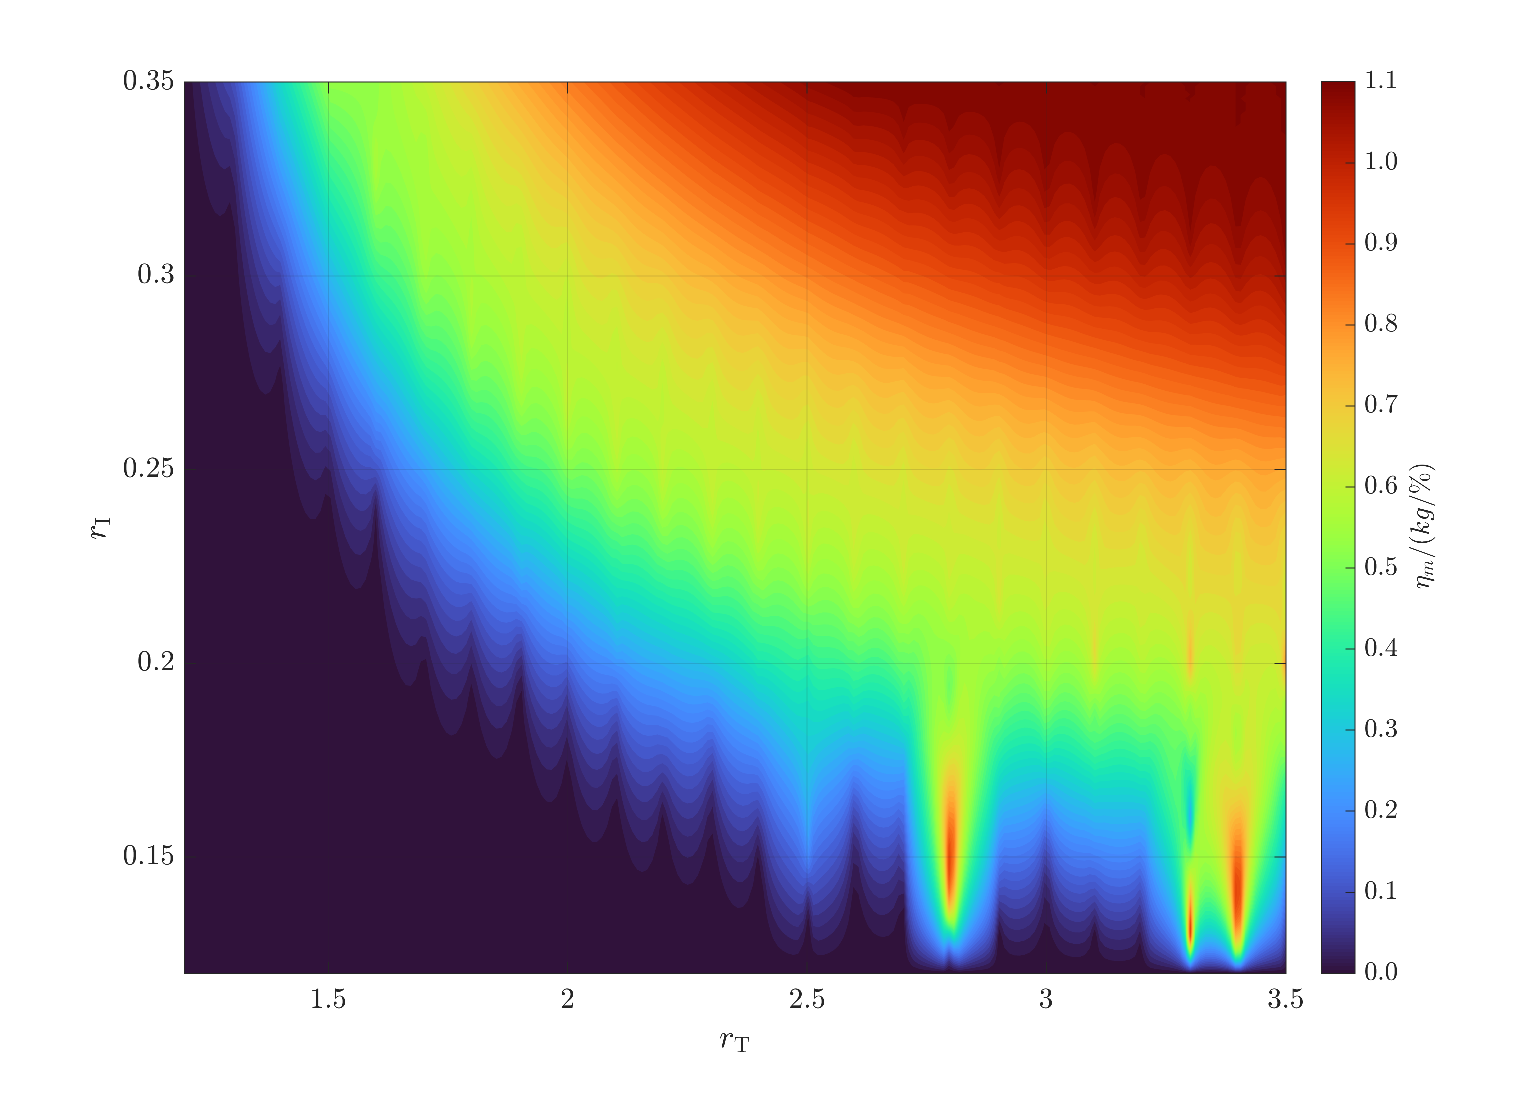
\includegraphics[width=0.98\columnwidth]{pdf_figures/fig3_12_gain_efficiency.pdf}
\caption{Mass-gain efficiency per unit non-low-thrust mode fraction.}
\label{fig:gain-efficiency}
\end{figure}

The preceding correlation analysis does not distinguish parameter combinations that obtain mass gain through relatively long non-low-thrust arcs from those that achieve comparable benefit with limited non-low-thrust usage. To quantify this effect, the mass-gain efficiency per unit non-low-thrust mode fraction is defined as
\begin{equation}
\eta_m=\frac{\Delta m_{\mathrm{f}}}{\rho}
\end{equation}
where the non-low-thrust mode fraction is
\begin{equation}
\rho=\frac{t_{\mathrm{c}}+t_2}{t_{\mathrm{tr}}}
\end{equation}
with $t_{\mathrm{c}}$ denoting the coasting time and $t_2$ denoting the high-thrust-mode operation time. The gain-efficiency plot measures how much terminal-mass benefit is obtained per unit non-low-thrust mode fraction under limited high-thrust or coasting usage. The high-efficiency region usually lies near the advantage boundary rather than in the upper-right region where the absolute gain is largest. For engineering selection, this implies that when the high-thrust mode is constrained by thermal control, power, or lifetime, parameter combinations near the boundary may be preferable to the maximum-gain point because they retain a measurable fuel benefit with a lower high-thrust usage fraction.

Combining the two-dimensional gain distribution, threshold curves, and efficiency distribution shows that terminal mass generally increases with the thrust ratio and specific-impulse ratio, but the non-low-thrust mode fraction $\rho$ is not fully synchronized with terminal mass. Some high-terminal-mass regions rely on relatively large coasting or high-thrust fractions, whereas some boundary regions obtain positive gain with limited use of non-low-thrust modes. This result has direct implications for single-thruster dual-mode design. If engineering constraints limit the operating duration of the high-thrust mode, mass-gain efficiency should be prioritized; if the mission emphasizes absolute propellant saving, parameter regions with both high thrust ratio and high specific-impulse ratio are preferable.

\section{Conclusions}
An indirect trajectory-optimization model was established for the Earth-to-Ceres fuel-optimal transfer using a single thruster with two operating modes. Typical trajectories, scheme comparisons, and propulsion-parameter boundaries were systematically analyzed through numerical simulations. The results show that the optimal control structure of the dual-mode coasting trajectory has a clear bang-off-bang characteristic. The high-specific-impulse low-thrust mode undertakes the main long-duration propulsion task, the high-thrust low-specific-impulse mode is concentrated in local arcs for rapid reconstruction of orbital energy and shape, and coasting arcs are used for phase waiting and for avoiding unnecessary propellant consumption.

The comparison among the four schemes indicates that the advantage of dual-mode propulsion should not be interpreted solely as having more operating modes. In a fixed-time fuel-optimal problem, coasting freedom is as important as mode switching. If the dual-mode system is forced to operate throughout the transfer, the additional mode may instead cause significant fuel loss during long-duration transfers. For the baseline propulsion parameters considered in this paper, the dual-mode coasting scheme has a clear advantage over the high-thrust-only scheme, whereas its benefit relative to the low-thrust-only scheme is small and concentrated in specific time windows. Thus, the value of dual-mode propulsion depends jointly on the mission time constraint and propulsion-parameter matching.

The analysis in the thrust-ratio-specific-impulse-ratio plane provides a critical boundary with clearer engineering interpretation. Compared with a single composite critical parameter, the two-dimensional boundary directly reveals the compensation relation between thrust enhancement and specific-impulse penalty: increasing the thrust ratio can reduce the specific-impulse ratio required for positive gain, but large fuel benefits still require the high-thrust mode to maintain a sufficiently high specific impulse. The analyses of mode fraction and mass-gain efficiency further show that the optimal benefit comes from the synergy among short high-thrust maneuvers, coasting for phase waiting, and high-specific-impulse continuous propulsion, rather than from a monotonic increase in high-thrust-mode operation time.

The main value of this work is to translate dual-mode optimal-control solutions into performance maps that can support mission design and preliminary propulsion-parameter selection. Although the theoretical framework builds on existing indirect-method and dual-mode optimal-control techniques, the asteroid exploration case clarifies how control freedom, the transfer-time parameter $\alpha_t$, and propulsion-parameter combinations jointly shape fuel performance. These results provide a simulation basis for subsequent dual-mode deep-space trajectory optimization and parameter-sensitivity analysis. Future work may incorporate higher-fidelity ephemeris models, engine operating constraints, and more robust homotopy strategies, especially near complex boundary regions and in multi-target or multiple-small-body transfer missions.


\bibliographystyle{IEEEtaes}
\bibliography{dualmode_refs}

\end{document}





